% =============================================================================
%  The D1 Arm, From Scratch — project book for D1T-Research
%  Built on the Packt-style technical book template (see git history for the
%  original template with usage notes).
%  COMPILE WITH:  latexmk -pdf main.tex   (or pdflatex twice)
% =============================================================================

\documentclass[11pt,twoside,openright]{book}

% ----------------------------------------------------------------------------
% 1. COLORS & FONTS
% ----------------------------------------------------------------------------
\usepackage[T1]{fontenc}
\usepackage[utf8]{inputenc}

\usepackage{xcolor}
\definecolor{accentorange}{HTML}{E8562F} % cover badge / chapter numbers / links
\definecolor{darkbg}{HTML}{1B1B1B}       % cover background
\definecolor{codebg}{HTML}{F2F2F2}       % code block background
\definecolor{noteborder}{HTML}{4D4D4D}   % note-box border
\definecolor{rulegray}{HTML}{999999}     % header/footer rule

\usepackage{mathpazo}      % serif body font
\usepackage{tgheros}       % sans-serif heading font
\usepackage[scaled]{beramono} % monospace font with a real bold weight
\renewcommand{\familydefault}{\rmdefault}

\usepackage{microtype}
\emergencystretch=1.5em

\definecolor{codekeyword}{HTML}{0B5394}
\definecolor{codestring}{HTML}{38761D}
\definecolor{codecomment}{HTML}{7F7F7F}

\newcommand{\headingfont}{\sffamily}
\newcommand{\code}[1]{\texttt{\bfseries #1}}

% ----------------------------------------------------------------------------
% 2. PAGE GEOMETRY
% ----------------------------------------------------------------------------
\usepackage[a4paper,inner=2.5cm,outer=2.2cm,top=2.3cm,bottom=2.5cm,headsep=14pt,headheight=22pt]{geometry}

% ----------------------------------------------------------------------------
% 3. CHAPTER / SECTION HEADING STYLES
% ----------------------------------------------------------------------------
\usepackage{titlesec}
\usepackage{titletoc}

\setcounter{secnumdepth}{0}

\titleformat{\chapter}[display]
  {\headingfont\bfseries}
  {\filright\fontsize{40}{40}\selectfont\color{accentorange}\thechapter}
  {6pt}
  {\Huge\bfseries\filright}
\titlespacing*{\chapter}{0pt}{-10pt}{30pt}

\titleformat{\section}
  {\headingfont\bfseries\Large}{}{0pt}{}
\titlespacing*{\section}{0pt}{22pt}{10pt}

\titleformat{\subsection}
  {\headingfont\bfseries\large}{}{0pt}{}
\titlespacing*{\subsection}{0pt}{16pt}{8pt}

\titleformat{\subsubsection}
  {\headingfont\bfseries\normalsize}{}{0pt}{}
\titlespacing*{\subsubsection}{0pt}{12pt}{6pt}

% ----------------------------------------------------------------------------
% 4. RUNNING HEADERS/FOOTERS
% ----------------------------------------------------------------------------
\usepackage{fancyhdr}

\renewcommand{\chaptermark}[1]{\markboth{#1}{}}
\renewcommand{\sectionmark}[1]{\markright{#1}{}}

\pagestyle{fancy}
\fancyhf{}
\renewcommand{\headrulewidth}{0.5pt}
\renewcommand{\footrulewidth}{0pt}
\renewcommand{\headrule}{\hbox to\headwidth{\color{rulegray}\leaders\hrule height \headrulewidth\hfill}}
\fancyhead[LE]{\small\thepage\hspace{1em}\leftmark}
\fancyhead[RO]{\small\rightmark\hspace{1em}\thepage}

\fancypagestyle{plain}{
  \fancyhf{}
  \fancyfoot[C]{\small\thepage}
  \renewcommand{\headrulewidth}{0pt}
}

\usepackage{emptypage}

% ----------------------------------------------------------------------------
% 5. NOTE / TIP BOX
% ----------------------------------------------------------------------------
\usepackage[most]{tcolorbox}
\newtcolorbox{pktbox}{
  enhanced, breakable,
  colback=white, colframe=noteborder,
  boxrule=0.6pt, arc=0pt,
  left=12pt, right=12pt, top=8pt, bottom=8pt,
  before skip=14pt plus 2pt, after skip=14pt plus 2pt,
}
\newenvironment{pktnote}{\begin{pktbox}\textbf{Note}\\[4pt]}{\end{pktbox}}
\newenvironment{pkttip}{\begin{pktbox}\textbf{Tip}\\[4pt]}{\end{pktbox}}
\newenvironment{pktimportant}{\begin{pktbox}\textbf{Important}\\[4pt]}{\end{pktbox}}

% Learning apparatus: prediction prompts and end-of-chapter retrieval questions
\newtcolorbox{pktpredictbox}{
  enhanced, breakable,
  colback=white, colframe=accentorange,
  boxrule=0.8pt, arc=0pt,
  left=12pt, right=12pt, top=8pt, bottom=8pt,
  before skip=14pt plus 2pt, after skip=14pt plus 2pt,
}
\newenvironment{pktpredict}{\begin{pktpredictbox}\textbf{\color{accentorange}Predict before reading on}\\[4pt]}{\end{pktpredictbox}}
\newenvironment{pktcheck}{%
  \section*{Check your understanding}%
  \addcontentsline{toc}{section}{Check your understanding}%
  \noindent Try these from memory before looking anything up --- recalling
  is the practice that makes it stick. Answers in Appendix~\ref{app:answers}.%
  \begin{enumerate}}{\end{enumerate}}

% ----------------------------------------------------------------------------
% 6. CODE BLOCK STYLE
% ----------------------------------------------------------------------------
\usepackage{listings}
\lstdefinestyle{pktcode}{
  backgroundcolor=\color{codebg},
  basicstyle=\ttfamily\bfseries\small,
  breaklines=true,
  breakatwhitespace=false,
  columns=fullflexible,
  keepspaces=true,
  showstringspaces=false,
  frame=single,
  rulecolor=\color{codebg},
  framerule=0pt,
  framesep=8pt,
  xleftmargin=0pt,
  xrightmargin=0pt,
  aboveskip=12pt,
  belowskip=12pt,
}
\lstset{style=pktcode}

\lstdefinestyle{pktsrc}{
  style=pktcode,
  basicstyle=\ttfamily\small,
  keywordstyle=\color{codekeyword}\bfseries,
  stringstyle=\color{codestring},
  commentstyle=\color{codecomment}\itshape,
  tabsize=4,
}
\lstdefinestyle{pktpython}{style=pktsrc, language=Python}
\lstdefinestyle{pktcpp}{style=pktsrc, language=C++}
\lstdefinestyle{pktyaml}{
  style=pktsrc,
  keywords={true,false,null},
  comment=[l]{\#},
  string=[b]",
  morestring=[b]',
}

\newcommand{\codefile}[1]{%
  \par\vspace{10pt}\noindent{\ttfamily\small\bfseries #1}\par\nopagebreak\vspace{-8pt}}

% ----------------------------------------------------------------------------
% 7. FIGURE CAPTION STYLE
% ----------------------------------------------------------------------------
\usepackage{graphicx}
\usepackage{tikz}
\usepackage[labelsep=endash,font=it,labelfont=it,justification=centering,skip=8pt]{caption}
\counterwithin{figure}{chapter}

\usepackage{enumitem}
\setlist[itemize]{topsep=6pt,itemsep=4pt,parsep=0pt,leftmargin=1.4em}
\setlist[enumerate]{topsep=6pt,itemsep=4pt,parsep=0pt,leftmargin=1.6em}

% ----------------------------------------------------------------------------
% Hyperref (load last)
% ----------------------------------------------------------------------------
\usepackage[colorlinks=true,linkcolor=black,citecolor=black,urlcolor=accentorange]{hyperref}
\hypersetup{
  pdftitle={The D1 Arm, From Scratch},
  pdfauthor={Ramiro Gonzalez},
  pdfsubject={Characterizing and controlling a Unitree D1 arm: the code, the experiments, and the robotics behind them},
}
\usepackage{bookmark}
\urlstyle{same}

\setcounter{tocdepth}{1}

\titlecontents{chapter}[0em]
  {\vspace{6pt}\bfseries}
  {\color{accentorange}\thecontentslabel\quad\color{black}}
  {}
  {\normalfont\bfseries\hfill\thecontentspage}
\titlecontents{section}[1.5em]
  {\vspace{2pt}}
  {}
  {}
  {\ \titlerule*[6pt]{.}\thecontentspage}
\titlecontents{subsection}[3em]
  {\vspace{1pt}}
  {}
  {}
  {\ \titlerule*[6pt]{.}\thecontentspage}

\begin{document}

% =============================================================================
% 8. FRONT MATTER
% =============================================================================

% ---- Cover page -------------------------------------------------------------
\begin{titlepage}
\newgeometry{margin=0cm}
\begin{tikzpicture}[remember picture,overlay]
  \fill[darkbg] (current page.north west) rectangle (current page.south east);

  % simple schematic arm as cover art
  \begin{scope}[shift={([yshift=-4cm]current page.north)},line cap=round]
    \draw[accentorange,line width=3pt] (-3.2,-1.6) -- (-1.6,0.4) -- (0.6,-0.4) -- (2.4,1.0);
    \fill[white] (-3.2,-1.6) circle (5pt);
    \fill[white] (-1.6,0.4) circle (5pt);
    \fill[white] (0.6,-0.4) circle (5pt);
    \fill[accentorange] (2.4,1.0) circle (5pt);
    \draw[white!40,line width=1pt] (-4.0,-1.6) -- (-2.4,-1.6);
  \end{scope}

  \node[white,font=\sffamily\bfseries,anchor=north east]
    at ([xshift=-1.2cm,yshift=-1cm]current page.north east) {D1T-RESEARCH};

  \node[fill=accentorange,text=white,font=\sffamily\bfseries\small,anchor=west,
        inner sep=6pt] at ([xshift=1.2cm,yshift=-7.3cm]current page.north west)
        {PROJECT BOOK};

  \node[white,font=\sffamily\bfseries\fontsize{48}{48}\selectfont,anchor=west,align=left]
    at ([xshift=1.2cm,yshift=-9.5cm]current page.north west) {THE D1 ARM,};
  \node[white,font=\sffamily\bfseries\fontsize{48}{48}\selectfont,anchor=west,align=left]
    at ([xshift=1.2cm,yshift=-10.8cm]current page.north west) {FROM SCRATCH};

  \node[white,font=\sffamily,anchor=west,align=left,text width=13cm]
    at ([xshift=1.2cm,yshift=-13cm]current page.north west)
    {Characterizing and controlling a Unitree D1 robot arm --- the code,
     the experiments, and the robotics ideas behind them};

  \node[white,font=\sffamily\bfseries\Large,anchor=south west]
    at ([xshift=1.2cm,yshift=1.2cm]current page.south west) {RAMIRO GONZALEZ};
\end{tikzpicture}
\end{titlepage}
\restoregeometry

% ---- Plain title page -------------------------------------------------------
\thispagestyle{empty}
\vspace*{4cm}
{\headingfont\bfseries\huge The D1 Arm, From Scratch\par}
\vspace{2cm}
{Characterizing and controlling a Unitree D1 robot arm --- the code,
the experiments, and the robotics ideas behind them\par}
\vspace{4cm}
{\headingfont\bfseries Ramiro Gonzalez\par}
\newpage

% ---- Colophon page ----------------------------------------------------------
% \repocommit is stamped by book/build.sh from git; fallback if built by hand.
\IfFileExists{gitrev.tex}{\input{gitrev.tex}}{}
\providecommand{\repocommit}{unversioned build}
\thispagestyle{empty}
{\headingfont\bfseries\large The D1 Arm, From Scratch\par}
\vspace{1em}
Copyright \copyright\ 2026 Ramiro Gonzalez

\vspace{1em}
Working documentation for the \code{D1T-Research} repository, intended to
be rebuilt at each phase freeze. This edition describes the system as of
July 2026 (end of Phase 2, Phase 3 tooling complete) and was built from
repository revision \code{\repocommit}. Code shown here is excerpted from
the repository; when the book and the repository disagree, \textbf{the
repository wins} on detail --- the book's job is the reasoning.

\vspace{1em}
\textbf{Hardware}: Unitree D1 arm (6 DOF + gripper) \\
\textbf{Workstation}: Ubuntu 26.04 LTS (Resolute Raccoon) \\
\textbf{ROS 2 (Phase 7 target)}: Lyrical Luth \\
\textbf{Theory text}: \textit{Modern Robotics}, Lynch \& Park \\
\textbf{Repository}: \code{D1T-Research}

\vspace{1em}
First assembled: July 2026

\newpage

% ---- Table of Contents ------------------------------------------------------
\thispagestyle{empty}
{\headingfont\bfseries\huge Table of Contents\par}
\vspace{1.5em}
\tableofcontents
\newpage

% ---- Preface ----------------------------------------------------------------
\chapter*{Preface}
\addcontentsline{toc}{chapter}{Preface}
\markboth{Preface}{Preface}

This book documents a year-long project: taking a Unitree D1 robot arm from
an unopened box to a full robotics stack --- forward kinematics, inverse
kinematics, ROS~2, trajectories, simulation, and perception --- with every
layer built and verified by hand on real hardware.

It exists for two reasons. First, as a record: six months from now it will
not be obvious why \code{j2} gets an extra $-0.6^\circ$ on negative targets,
or why the logger starts two seconds before every command. The answers are
in the data, and this book explains them. Second, as a teaching document:
everything here was learned while doing it, and the book is written so that
someone starting from general programming knowledge --- but no robotics ---
can understand not just \emph{what} the code does but \emph{why} it is
shaped the way it is.

The guiding rule of the whole project is borrowed from experimental science:
\textbf{verify before optimize --- if it's not measured, it's not real.}
Commanded angles are not measured angles. Datasheets are not ground truth.
Every phase of the project produces raw logs, a script that analyzes them,
and a written record of what was found.

\section*{Who this book is for}

Anyone in or around robotics who wants to see what careful,
from-first-principles work looks like on hobbyist-priced hardware:
software engineers moving toward robotics, technicians and students who
have driven arms but not characterized one, D1 owners looking for a map
past the vendor examples, and the future maintainer of this repository.
Everything here generalizes --- the step-response method, the safety
contract, the bridge architecture --- and the D1 is simply the concrete
arm it is demonstrated on: real telemetry, real safety constraints, and
real firmware quirks discovered by measurement.

You should be comfortable with Python and a terminal. No robotics
background is assumed: every concept (DDS, deadband, step response, screw
axes) is introduced when it first earns its keep. C++ appears only in
one short bridge program, explained line by line. The robotics math (screw
theory, Jacobians) is introduced conceptually in Chapter~\ref{ch:road} before the phases
that need it.

\section*{How to use this book}

The book is built around how technical memory actually forms, and two
recurring elements ask for a little active work:

\begin{itemize}
  \item \textbf{``Predict before reading on'' boxes} pose a question just
    before the text answers it. Stop and commit to an answer --- even a
    wrong guess measurably improves how well the explanation that follows
    sticks. They are placed at the points where this project itself had
    to stop and reason.
  \item \textbf{``Check your understanding'' questions} close every
    chapter. They are retrieval practice, not review: attempt them from
    memory first, then check Appendix~\ref{app:answers}. Recalling an
    idea strengthens it far more than re-reading it, so the questions are
    the highest-value minutes in each chapter.
\end{itemize}

Readers with an arm on the desk get the most transfer by running each
chapter's commands as they read; readers without one lose surprisingly
little, because every experiment's raw data and plots are in the
repository.

\section*{A note on change}

The repository is alive: file names, command-line flags, pose tables, and
thresholds will drift as the phases advance, and this book will
periodically be behind. That is expected and managed rather than fought:

\begin{itemize}
  \item \textbf{Concepts over coordinates.} Chapters lead with ideas that
    do not expire --- step response, deadband, path dependence, screw
    axes, pub/sub --- and use today's code as the worked example. If a
    file is renamed, read the excerpt for its \emph{role} (``the pose
    sender'', ``the limits contract'') and find the current file playing
    that role.
  \item \textbf{Volatile detail lives in one place.} Exact commands,
    filenames, versions, and measured constants are concentrated in
    Appendix~A, so keeping the book current means revising one appendix,
    not seven chapters.
  \item \textbf{Editions track phase freezes.} The book is rebuilt at
    each phase tag, and the colophon records the exact repository
    revision an edition describes. For the true state of any detail,
    check out that revision --- the repository always wins.
\end{itemize}

\section*{What this book covers}

\noindent\textbf{Chapter \ref{ch:project}, \textit{The Project and the
Plan}}, sets out the goal, the eleven-phase roadmap, the rules of work,
and a tour of the repository.

\noindent\textbf{Chapter \ref{ch:setup}, \textit{From Box to First
Motion}}, is the hands-on setup guide: hardware, Ubuntu 26.04, the SDK
build, ROS~2 Lyrical Luth, the power-on ritual, and a verified first
move --- with troubleshooting.

\noindent\textbf{Chapter \ref{ch:talking}, \textit{Talking to the Arm}},
explains the communication stack: Ethernet, DDS publish/subscribe, and the
JSON command protocol the arm actually speaks.

\noindent\textbf{Chapter \ref{ch:bridge}, \textit{The C++/Python
Bridge}}, walks through the two small C++ programs that connect Python to
the robot, and the architecture decision behind them.

\noindent\textbf{Chapter \ref{ch:toolkit}, \textit{The Experiment
Toolkit}}, covers the Python tools every experiment uses: the telemetry
logger, the pose sender, and the safety-limits module.

\noindent\textbf{Chapter \ref{ch:phase2}, \textit{Phase 2 --- What the
Joints Actually Do}}, presents the single-joint characterization campaign:
step responses, settle times, zero offsets, and the discovery of a
controller deadband.

\noindent\textbf{Chapter \ref{ch:phase3}, \textit{Phase 3 --- The Safe
Envelope}}, covers multi-joint testing: named poses, sequence runs,
path-dependence analysis, and the \code{limits.py} contract that all later
phases import.

\noindent\textbf{Chapter \ref{ch:road}, \textit{The Road Ahead}}, previews
the robotics theory of Phases 4--11 --- kinematics, Jacobians, IK, ROS~2,
trajectories, simulation, perception --- and what to read for each.

\noindent\textbf{Appendix A, \textit{Quick Reference}}, is the cheat sheet:
commands, file map, and protocol tables.

\noindent\textbf{Appendix B, \textit{Answers}}, holds the answers to every
chapter's ``Check your understanding'' questions.

\newpage

% =============================================================================
% CHAPTER
% =============================================================================

\chapter{The Project and the Plan}\label{ch:project}

A robot arm on a desk is a promise, not a capability. Out of the box, the
Unitree D1 will move to angles you send it --- but it will not tell you how
accurately, how repeatably, or how safely. The gap between ``it moves'' and
``I can build a manipulation system on it'' is precisely the work this
project does, and this chapter explains how that work is organized.

\section{The goal}

The end state, targeted for mid-2027, is a complete perception-guided
pick-and-place system: a camera detects an object, inverse kinematics ---
implemented from the math, not from a library --- plans a reach, a
trajectory generator executes it smoothly, and ROS~2 ties it all together.
Every layer is validated on real hardware and published as a reproducible
portfolio.

That target was chosen deliberately. Surveying what robotics employers ask
for produces a consistent list, and the project phases map onto it directly:

\begin{itemize}
  \item \textbf{ROS 2} (pub/sub, actions, tf2) --- in roughly 90\% of job
    postings; covered by Phase 7.
  \item \textbf{FK / IK from scratch} --- demonstrates mathematical depth;
    Phases 4--6.
  \item \textbf{Trajectory planning} --- Phase 8.
  \item \textbf{Simulation} (MuJoCo / Gazebo) --- sim-to-real workflows;
    Phase 9.
  \item \textbf{Perception} --- the top skill gap in manipulation;
    Phase 10.
  \item \textbf{Real hardware demos} --- what separates hardware people
    from pure-simulation people; every phase here runs on the real arm.
\end{itemize}

\section{The eleven phases}

The roadmap lives in \code{yearplan.md} and is the single source of truth
for scope. One phase is active at a time; a closed phase only reopens with
evidence that something it produced is wrong.

\begin{enumerate}
  \item \textbf{Phase 0--1} --- OS setup, network bring-up, logging, zero
    and reference integrity. \emph{Done.}
  \item \textbf{Phase 2} --- single-joint characterization: what does each
    joint actually do when commanded? \emph{Done; results in Chapter~\ref{ch:phase2}.}
  \item \textbf{Phase 3} --- multi-joint coordination and the safe
    envelope. \emph{Tooling complete; hardware runs in progress
    (Chapter~\ref{ch:phase3}).}
  \item \textbf{Phases 4--6} --- forward kinematics, Jacobians,
    numerical IK, all implemented from \textit{Modern Robotics} (Lynch \&
    Park) and validated physically.
  \item \textbf{Phase 7} --- ROS 2 integration; the stdin/stdout bridge is
    replaced by proper nodes and topics.
  \item \textbf{Phases 8--10} --- trajectories and gravity compensation,
    simulation, camera perception.
  \item \textbf{Phase 11} --- the capstone pick-and-place, measured over
    20 trials.
\end{enumerate}

\section{The rules of work}

Five rules govern every phase. They sound obvious; the discipline is in
actually following them.

\begin{itemize}
  \item \textbf{Verify before optimize.} If it's not measured, it's not
    real.
  \item \textbf{One variable per experiment.} Phase 2 moves one joint at a
    time for exactly this reason.
  \item \textbf{Freeze means freeze.} Each phase ends with a tagged commit
    and archived logs. Raw logs are immutable.
  \item \textbf{Every phase produces a public artifact} --- code, a plot,
    and a short write-up.
  \item \textbf{Safety first.} If the arm strains, sounds different, or
    hits anything, that angle is out of bounds and gets documented. Never
    test near joint limits.
\end{itemize}

\section{The hardware: D1-550 in numbers}

The arm is a Unitree \textbf{D1-550} (the D1-T kit pairs two of them ---
more on that in Chapter~\ref{ch:setup}). The numbers that shape this
project, from the official specification:

\begin{itemize}
  \item \textbf{Geometry}: 550\,mm arm length (670\,mm with gripper),
    550\,mm working radius, 3.15\,kg total weight.
  \item \textbf{Payload}: 500\,g rated load \emph{including} the gripper
    jaws --- a light-duty arm; gravity effects matter (Phase 8).
  \item \textbf{Joint torque}: 3.3\,Nm on j0 and j1, 1.7\,Nm on the
    rest. j1 carries the arm's own weight at reach, which is why it is
    the prime candidate for gravity compensation.
  \item \textbf{Factory range of motion}: $\pm135^\circ$ on j0, j3, j5;
    $\pm90^\circ$ on j1, j2, j4; 0--65\,mm claw stroke on j6. This
    project's conservative envelope ($\pm45^\circ$, Chapter
    \ref{ch:phase3}) sits far inside these --- deliberately. Never test
    near the factory limits.
  \item \textbf{Control}: onboard controller (4$\times$ Cortex-A55),
    DDS subscription over 100\,Mbps Ethernet, \textbf{10\,Hz control
    cycle} --- the same 10\,Hz seen in the telemetry stream and the
    streaming command mode.
  \item \textbf{Power}: 24\,V / 10\,A supply (240\,W).
\end{itemize}

\section{A tour of the repository}

\begin{lstlisting}
D1T-Research/
  setup.sh           one-command machine setup: network, NIC patch, build
  yearplan.md        the eleven-phase roadmap (source of truth for scope)
  d1_guide.ipynb     narrative guide: hardware -> setup -> commands
  d1_sdk/
    src/             C++ programs that speak DDS to the arm
    build/           compiled binaries
    PROTOCOL.md      the arm's JSON command protocol, documented
  experiments/       Python: loggers, pose tools, phase scripts, results
  logs/              raw telemetry CSVs, one folder per phase (immutable)
  90b2525.../        URDF + meshes, needed from Phase 4 onward
  ROS2/              ROS 2 study notes for Phase 7
  book/              this book
\end{lstlisting}

The split matters: \code{d1\_sdk/} is the only place C++ lives,
\code{experiments/} is where all science happens, and \code{logs/} is
write-once. Analysis scripts read logs; they never edit them.

\begin{figure}[tb]
\centering
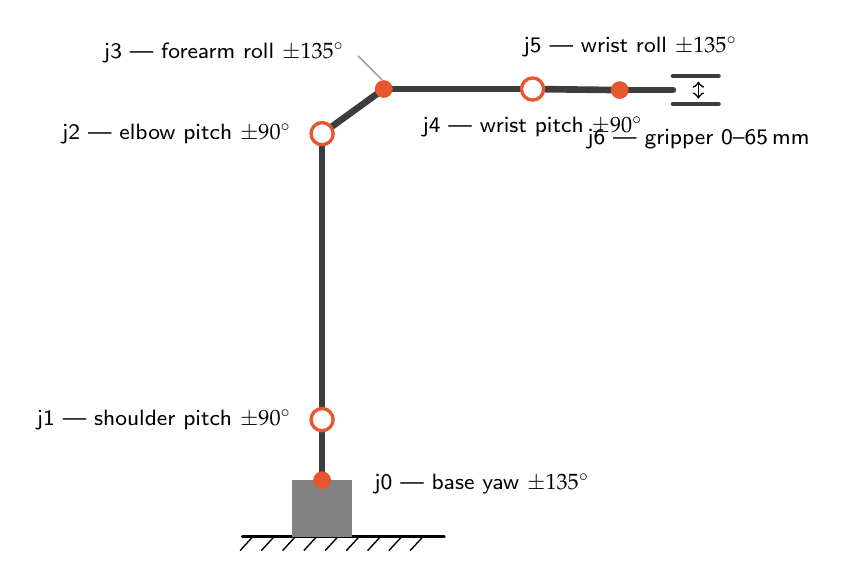
\begin{tikzpicture}[scale=13.5,line cap=round,
  jlabel/.style={font=\footnotesize\sffamily},
  link/.style={line width=2.4pt,darkbg!85},
  pitchj/.style={circle,draw=accentorange,fill=white,line width=1.2pt,
                 inner sep=0pt,minimum size=8pt},
  rollj/.style={circle,draw=accentorange,fill=accentorange,
                inner sep=0pt,minimum size=6pt}]

  % ground
  \draw[line width=1pt] (-0.075,0) -- (0.115,0);
  \foreach \gx in {-0.065,-0.045,...,0.106}
    \draw[line width=0.5pt] (\gx,0) -- (\gx-0.012,-0.013);

  % base column
  \fill[darkbg!55] (-0.028,0) rectangle (0.028,0.053);

  % links (URDF joint origins, zero configuration)
  \draw[link] (0,0.053) -- (0,0.110);
  \draw[link] (0,0.110) -- (0,0.379);
  \draw[link] (0,0.379) -- (0.058,0.421);
  \draw[link] (0.058,0.421) -- (0.198,0.421);
  \draw[link] (0.198,0.421) -- (0.280,0.420);
  \draw[link] (0.280,0.420) -- (0.330,0.420);

  % gripper jaws (prismatic)
  \draw[line width=1.6pt,darkbg!85] (0.330,0.433) -- (0.373,0.433);
  \draw[line width=1.6pt,darkbg!85] (0.330,0.407) -- (0.373,0.407);
  \draw[<->,line width=0.6pt] (0.354,0.428) -- (0.354,0.412);

  % joints
  \node[rollj]  at (0,0.053) {};
  \node[pitchj] at (0,0.110) {};
  \node[pitchj] at (0,0.379) {};
  \node[rollj]  at (0.058,0.421) {};
  \node[pitchj] at (0.198,0.421) {};
  \node[rollj]  at (0.280,0.420) {};

  % labels
  \node[jlabel,anchor=west]  at (0.040,0.050)  {j0 --- base yaw $\pm135^\circ$};
  \node[jlabel,anchor=east]  at (-0.020,0.110) {j1 --- shoulder pitch $\pm90^\circ$};
  \node[jlabel,anchor=east]  at (-0.020,0.379) {j2 --- elbow pitch $\pm90^\circ$};
  \node[jlabel,anchor=east]  at (0.030,0.455)  {j3 --- forearm roll $\pm135^\circ$};
  \draw[line width=0.5pt,rulegray] (0.056,0.430) -- (0.034,0.452);
  \node[jlabel,anchor=north] at (0.198,0.404)  {j4 --- wrist pitch $\pm90^\circ$};
  \node[jlabel,anchor=south] at (0.290,0.442)  {j5 --- wrist roll $\pm135^\circ$};
  \node[jlabel,anchor=north] at (0.354,0.392)  {j6 --- gripper 0--65\,mm};
\end{tikzpicture}
\caption{The D1-550 at its zero configuration, side view, drawn to scale
from the joint origins in the repository's URDF. The zero posture is an
L: upper arm vertical, forearm horizontal. Open circles are pitch joints
(axes into the page); filled circles rotate about the vertical (j0) or
about the link axis (j3, j5); the jaws (j6) are prismatic sliders ---
a linear stroke, not a rotation.}
\label{fig:arm}
\end{figure}

\begin{pktnote}
The D1 is 6 DOF plus a gripper, and the wire protocol exposes
\textbf{seven} angle channels. The official numbering runs from the base
(Figure~\ref{fig:arm}): \code{j0} (base yaw) through \code{j5} are the six
arm joints, and \code{j6} drives the gripper --- a 0--65\,mm claw stroke
behind an angle channel; the URDF models it as prismatic slider joints.
This project's tooling treats all seven channels uniformly; the
kinematics phases operate on \code{j0}--\code{j5}.
\end{pktnote}

\section*{Summary}
\addcontentsline{toc}{section}{Summary}

The project turns a bare D1 arm into a validated robotics stack over eleven
phases, each producing measured evidence before the next begins. The
repository separates C++ robot I/O, Python experiments, and immutable logs.
With the map in hand, the next chapter gets you from an unopened box to a
verified first motion.

\begin{pktcheck}
  \item The wire protocol exposes seven angle channels. Which are true
    rotations, and what is the seventh actually driving?
  \item Two joints have 3.3\,Nm of torque; the rest have 1.7\,Nm. Which
    two, and why does the asymmetry matter once the arm is extended?
  \item Why is \code{logs/} write-once? What is an analysis script
    allowed to do with a log file, and what is it never allowed to do?
  \item From memory: where in the repository do C++ code, Python
    experiments, and raw data live --- and what is the argument for
    keeping them separated?
\end{pktcheck}

% =============================================================================
% CHAPTER
% =============================================================================

\chapter{From Box to First Motion}\label{ch:setup}

This chapter is the complete setup path: hardware on the desk, a fresh
Ubuntu 26.04 install, through to the arm verifiably obeying a command. It
assumes nothing beyond a working OS and follows the exact order that
avoids the common traps. If a step fails, jump to the troubleshooting
section at the end before improvising.

\section{Technical requirements}

\begin{itemize}
  \item \textbf{Unitree D1-550 arm} with its 24\,V power supply (the
    D1-T kit contains two arms; one is enough for everything before the
    teleoperation experiments --- see the D1-T section below).
  \item \textbf{An Ethernet path} between workstation and arm: a built-in
    port or a USB-C/USB-A Ethernet adapter --- both work, and
    \code{setup.sh} auto-detects either.
  \item \textbf{Workstation with Ubuntu 26.04 LTS} (Resolute Raccoon),
    with sudo rights and internet access for the installs.
  \item \textbf{A clear workspace}: the arm bolted or clamped to a
    surface, with a full arm's reach of empty space around it --- no
    monitors, mugs, or cables inside the sweep.
\end{itemize}

\begin{pktimportant}
Set up the physical safety habit before the software: know where the
power switch is, and keep a hand's reach to it during every first-time
motion. An arm doing something unexpected is stopped with power, not with
Ctrl-C --- the arm's controller, not your process, is executing the move.
\end{pktimportant}

\section{Step 1 --- physical setup}

\begin{enumerate}
  \item Mount the arm on a stable surface. It must not be able to tip or
    walk when moving at full extension.
  \item Connect the Ethernet cable from the arm to the workstation (or
    to the USB adapter).
  \item Connect power but leave the arm \textbf{off} for now --- the
    software side comes first, so that telemetry is watchable the moment
    the arm boots.
\end{enumerate}

\section{Step 2 --- install unitree\_sdk2}

The arm's SDK examples build against \code{unitree\_sdk2}, which also
provides CycloneDDS (the middleware explained in
Chapter~\ref{ch:talking}). This is a one-time system-wide install:

\begin{lstlisting}
$ sudo apt update
$ sudo apt install -y build-essential cmake git
$ git clone https://github.com/unitreerobotics/unitree_sdk2
$ cd unitree_sdk2 && mkdir build && cd build
$ cmake .. && sudo make install
\end{lstlisting}

\section{Step 3 --- clone and run setup.sh}

\begin{lstlisting}
$ git clone <this-repo-url> D1T-Research
$ cd D1T-Research
$ ./setup.sh
\end{lstlisting}

The script is idempotent --- safe to re-run at any time --- and does four
jobs, printing a check mark per step:

\begin{enumerate}
  \item Installs any missing system packages (compiler, cmake,
    NetworkManager tools).
  \item Auto-detects the Ethernet interface facing the arm and writes a
    static IP profile named \code{d1-robot}: host
    \code{192.168.123.10}, robot at \code{192.168.123.100}.
  \item Patches the detected interface name into every SDK source file
    (the DDS layer binds to the interface by name --- see
    Chapter~\ref{ch:talking} for why).
  \item Builds all binaries into \code{d1\_sdk/build/}.
\end{enumerate}

Also install the Python analysis stack used by every experiment:

\begin{lstlisting}
$ pip install numpy matplotlib pandas
\end{lstlisting}

\begin{pkttip}
Swapped to a different USB Ethernet adapter? The interface name changed
with it. Just re-run \code{./setup.sh}; re-detection and re-patching is
the supported workflow.
\end{pkttip}

\section{Step 4 --- install ROS 2 Lyrical Luth}

ROS 2 is not needed until Phase 7, but installing it during setup is
cheap and makes the machine future-complete. Ubuntu 26.04 pairs with the
\textbf{Lyrical Luth} distribution; use the official binary packages
(never build ROS from source for this project), following the current
instructions at \code{docs.ros.org} for Lyrical Luth. The shape of the
install:

\begin{lstlisting}
$ sudo apt install ros-lyrical-desktop
$ sudo apt install python3-colcon-common-extensions
$ echo "source /opt/ros/lyrical/setup.bash" >> ~/.bashrc
\end{lstlisting}

Verify with \code{ros2 topic list} in a fresh terminal --- it should run
without error (and show only default topics for now). Nothing else in
this book touches ROS 2 until Phase 7.

\begin{pktpredict}
Software is installed and the arm is about to be powered for the first
time. Three first actions are available: read telemetry, enable the
motors, or send a motion command. Decide on the safest order --- and why
a motion command is the wrong \emph{first} test --- before reading the
checklist below.
\end{pktpredict}

\section{Step 5 --- power on and verify, in order}

Switch the arm on and \textbf{wait 60--90 seconds} --- the controller
boots slower than feels natural, and commands sent early vanish silently.
Then verify in this exact order, from \code{d1\_sdk/build/}:

\begin{enumerate}
  \item \textbf{Telemetry first} --- prove you can \emph{hear} the arm
    before asking it to do anything:
\begin{lstlisting}
$ ./get_arm_joint_angle
servo0_data:0.1, servo1_data:0.4, ... servo6_data:-0.2
\end{lstlisting}
    A stream of lines like this at roughly 10 per second means the
    network, DDS, and arm are all alive. No lines? Troubleshooting
    section, entry 1.
  \item \textbf{Enable the joints} (locks the motors so they hold
    position): \code{./joint\_enable\_control}
  \item \textbf{Zero the arm}: \code{./arm\_zero\_control} --- the arm
    moves smoothly to its zero posture. Watch it; this is the first
    motion.
\end{enumerate}

\section{Step 6 --- first commanded move}

Do the first real move through the Python tooling, not raw binaries,
because it validates angles against the safe limits before sending
(Chapter~\ref{ch:toolkit} explains the machinery):

\begin{lstlisting}
$ python experiments/send_pose.py reach_1
Sent: j0=0  j1=-5  j2=10  j3=0  j4=5  j5=0  j6=0
$ python experiments/send_pose.py zero
\end{lstlisting}

The arm should ease into a slight reach and back. If it did, the whole
stack works end to end, and everything else in this book is available to
you. New machines end here; a new \emph{arm} should also get the Phase 2
characterization re-run (Chapter~\ref{ch:phase2}) --- offsets and
deadbands are per-unit facts, not model facts.

\section{About the D1-T dual-arm kit}

\textbf{D1-T} is Unitree's teleoperation bundle: \emph{two} D1-550 arms
--- an \emph{acquisition} arm fitted with a hand-held claw (you move it,
it streams its joint angles) and an \emph{execution} arm that mirrors
them --- networked through a router. Useful facts from the official docs,
even for single-arm work:

\begin{itemize}
  \item \textbf{Every arm ships at} \code{192.168.123.100}. To run two
    on one network, SSH into one (\code{ssh ubuntu@192.168.123.100},
    password \code{123}) and change its IP in \code{/etc/network} ---
    the convention is \code{.99} for the second arm.
  \item \textbf{The arm is itself a Linux box} running Unitree's
    \code{marm\_*} services (\code{controller}, \code{control},
    \code{communication}, \code{subscripber}); they can be stopped,
    disabled, or --- for multi-arm setups on one router --- rebuilt with
    per-arm topic names by editing \code{marm\_code/src} on the arm.
  \item \textbf{Two ways to address two arms}: separate NICs on the
    workstation with one arm each (bind by interface name, exactly the
    \code{Init(0, "...")} pattern this repository already uses), or
    unique DDS topics per arm when everything shares one router.
\end{itemize}

This project runs a single arm in the execution-arm configuration, with
its factory services untouched. The teleoperation and dual-arm workflows
become relevant only if a data-collection phase (drag teaching,
demonstrations) is added later.

\section{Troubleshooting}

\begin{enumerate}
  \item \textbf{No telemetry lines.} In order: is the arm's boot wait
    over? Link up (\code{ip link} shows the interface \code{UP})? Can
    you \code{ping 192.168.123.100}? If ping works but there is still no
    data, the binary is bound to a stale interface name --- re-run
    \code{./setup.sh} and rebuild. This one cause explains nearly every
    ``program runs, nothing happens''.
  \item \textbf{Build fails with missing unitree headers.} Step 2 was
    skipped or failed --- \code{unitree\_sdk2} must be installed
    system-wide before \code{setup.sh} can build.
  \item \textbf{Arm ignores move commands but telemetry works.} Joints
    are not enabled --- run \code{./joint\_enable\_control} after every
    arm power cycle.
  \item \textbf{send\_pose.py rejects an angle.} Working as intended:
    the pose violates \code{limits.py}. Read
    Chapter~\ref{ch:phase3} before considering widening a bound.
  \item \textbf{Arm does something unexpected.} Power off first, ask
    questions after. Then check the workspace, re-zero, and if anything
    sounded or looked wrong, record it --- that is data
    (Chapter~\ref{ch:phase3}'s safety rule).
\end{enumerate}

\section*{Summary}
\addcontentsline{toc}{section}{Summary}

One SDK install, one script, one ordered verification: hear the arm, lock
it, zero it, then command it through the validated Python path. The
machine is now equipped through Phase 7's ROS 2 needs. The next chapter
explains what was actually happening under those commands --- the
network, the middleware, and the protocol.

\begin{pktcheck}
  \item After powering the arm, what gets verified first --- and why
    that, before anything is commanded?
  \item Why is Ctrl-C not an emergency stop for this arm, and what is?
  \item ``The program runs but nothing happens.'' What is the most likely
    cause, and what fixes it?
  \item A new arm (not a new computer) arrives. Which procedure must be
    re-run, and why don't the old measured constants carry over?
\end{pktcheck}

% =============================================================================
% CHAPTER
% =============================================================================

\chapter{Talking to the Arm}\label{ch:talking}

Every capability this project builds --- characterization, kinematics,
trajectories --- ultimately becomes a string of JSON pushed over Ethernet.
This chapter explains that pipe from the wire up: the network link, the DDS
middleware, and the arm's JSON protocol.

\section{The physical link}

The D1 connects to the workstation over Ethernet and lives at a fixed
address on a private subnet:

\begin{itemize}
  \item \textbf{Robot}: \code{192.168.123.100}
  \item \textbf{Host}: \code{192.168.123.10}, configured as a static
    profile named \code{d1-robot} by \code{setup.sh}
\end{itemize}

\code{setup.sh} is the one-command bring-up for a fresh machine. It
installs missing packages, verifies the \code{unitree\_sdk2} headers and
CycloneDDS are installed, auto-detects which Ethernet interface is the
robot link (it works with built-in ports and USB-C adapters), writes the
static IP profile, and builds the SDK programs. It is safe to re-run at any
time --- swapping to a different USB Ethernet adapter and re-running
\code{./setup.sh} is the supported workflow.

\begin{pktimportant}
Every C++ program binds DDS to the robot's network interface
\emph{explicitly}, by name:

\code{ChannelFactory::Instance()->Init(0, "enx4cea4168e514");}

Interface names like \code{enx4cea4168e514} are derived from the adapter's
MAC address, so they change when the adapter does. \code{setup.sh} patches
the current name into the sources automatically; a mysterious ``program
runs but nothing happens'' is almost always a stale interface name.
\end{pktimportant}

\section{DDS in one page}

The D1 does not expose a REST API or a serial protocol. It speaks
\textbf{DDS} (Data Distribution Service), the same publish/subscribe
middleware that underlies ROS~2 --- one reason this project's later ROS~2
phase is a natural fit.

The mental model:

\begin{itemize}
  \item \textbf{Topic}: a named channel, like a radio frequency. Writers
    publish onto it; readers subscribe to it. Nobody connects to anybody
    directly.
  \item \textbf{No broker}: there is no central server. Participants
    discover each other by multicast on the local network segment ---
    which is why the interface binding above matters.
  \item \textbf{Typed messages}: each topic carries one message type. The
    arm uses two: \code{ArmString\_} (a wrapper around a JSON string) and
    \code{PubServoInfo\_} (a struct of seven floats).
\end{itemize}

Three topics matter (Figure~\ref{fig:dds}):

\begin{itemize}
  \item \code{rt/arm\_Command} --- host publishes JSON commands here.
  \item \code{arm\_Feedback} --- arm publishes JSON status and
    acknowledgements here.
  \item \code{current\_servo\_angle} --- arm publishes raw per-servo
    angles here at about 10\,Hz, as \code{PubServoInfo\_} structs.
\end{itemize}

\begin{figure}[tb]
\centering
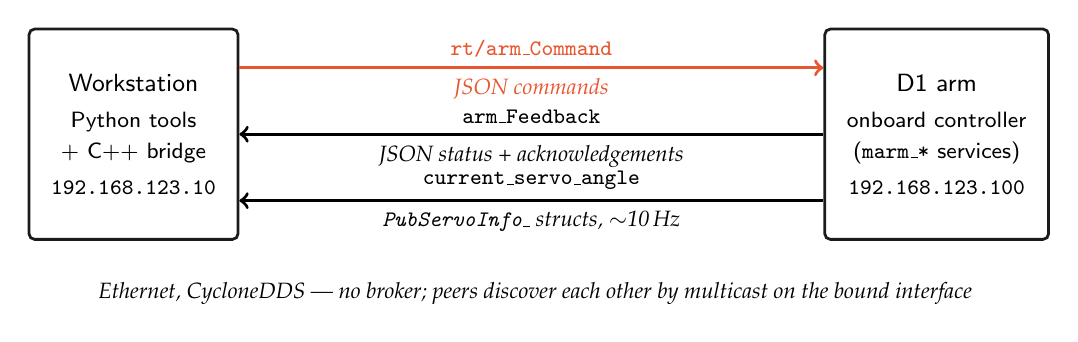
\begin{tikzpicture}[font=\small\sffamily,
  box/.style={draw=darkbg,line width=1pt,rounded corners=2pt,
              align=center,inner sep=8pt,minimum height=76pt},
  topic/.style={font=\footnotesize\ttfamily\bfseries},
  note/.style={font=\footnotesize\itshape}]
  \node[box] (host) at (0,0)
    {Workstation\\[2pt]
     \footnotesize Python tools\\
     \footnotesize + C++ bridge\\[2pt]
     \footnotesize\ttfamily 192.168.123.10};
  \node[box] (arm) at (10.2,0)
    {D1 arm\\[2pt]
     \footnotesize onboard controller\\
     \footnotesize (\ttfamily marm\_*\sffamily\ services)\\[2pt]
     \footnotesize\ttfamily 192.168.123.100};
  \draw[->,line width=1.2pt,accentorange]
    ([yshift=24pt]host.east) -- ([yshift=24pt]arm.west)
    node[topic,above,midway]{rt/arm\_Command}
    node[note,below,midway]{JSON commands};
  \draw[<-,line width=1.2pt]
    (host.east) -- (arm.west)
    node[topic,above,midway]{arm\_Feedback}
    node[note,below,midway]{JSON status + acknowledgements};
  \draw[<-,line width=1.2pt]
    ([yshift=-24pt]host.east) -- ([yshift=-24pt]arm.west)
    node[topic,above,midway]{current\_servo\_angle}
    node[note,below,midway]{\code{PubServoInfo\_} structs, $\sim$10\,Hz};
  \node[note,anchor=north] at (5.1,-1.75)
    {Ethernet, CycloneDDS --- no broker; peers discover each other by
     multicast on the bound interface};
\end{tikzpicture}
\caption{The complete communication surface between workstation and arm:
one topic of commands in, two topics of telemetry out. There is no
central server --- which is why every program must bind to the correct
network interface by name.}
\label{fig:dds}
\end{figure}

The concrete DDS implementation is Eclipse CycloneDDS, installed as part
of \code{unitree\_sdk2}. The Unitree SDK wraps it in two small classes ---
\code{ChannelPublisher} and \code{ChannelSubscriber} --- which are the only
DDS API this project touches.

\section{The JSON protocol}

Inside every \code{ArmString\_} message is a JSON object with the same
four-field envelope, fully documented in \code{d1\_sdk/PROTOCOL.md}:

\begin{lstlisting}[style=pktyaml]
{"seq": 4, "address": 1, "funcode": 1, "data": { ... }}
\end{lstlisting}

\begin{itemize}
  \item \textbf{seq}: a tag you choose for commands (the examples all use
    4). Feedback the arm volunteers uses \code{seq = 10};
    acknowledgements echo the \code{seq} of the command they answer, which
    is how you match replies to requests.
  \item \textbf{address}: which subsystem --- \code{1} = commands to the
    arm, \code{2} = continuous state feedback from the arm, \code{3} =
    per-command acknowledgements from the arm.
  \item \textbf{funcode}: the instruction within that subsystem.
  \item \textbf{data}: the payload; its shape depends on the funcode.
\end{itemize}

\subsection{Commands (address 1)}

\begin{itemize}
  \item \textbf{funcode 1} --- single-joint move: \code{id},
    \code{angle}, \code{delay\_ms} (currently unused, send 0).
  \item \textbf{funcode 2} --- all-joint move: \code{mode} plus
    \code{angle0}\ldots\code{angle6}. Mode 0 means smoothed 10\,Hz
    streaming updates; mode 1 means a trajectory-style move with large
    smoothing. \emph{This is the workhorse; everything in this project
    sends funcode 2, mode 1.}
  \item \textbf{funcode 4 / 5} --- enable or de-energize one joint / all
    joints. Nominally \code{mode} 1 = enable, 0 = free, but the official
    docs reveal it is really a \emph{lock level} from 0 (fully unloaded)
    to 80000 (fully locked) --- a dial, not a switch. De-energized
    joints plus the angle feedback stream enable \textbf{drag teaching}:
    physically move the arm and record the angles as a demonstration.
  \item \textbf{funcode 6} --- motor power switch. Doubles as the
    software emergency stop.
  \item \textbf{funcode 7} --- return to zero posture; takes no
    \code{data} at all.
\end{itemize}

A complete all-joint command looks like this:

\begin{lstlisting}[style=pktyaml]
{"seq":4,"address":1,"funcode":2,"data":{"mode":1,
 "angle0":0,"angle1":-30,"angle2":30,"angle3":0,
 "angle4":20,"angle5":0,"angle6":0}}
\end{lstlisting}

\subsection{Feedback (address 2) and acknowledgements (address 3)}

On \code{address 2} the arm continuously pushes joint angles
(funcode 1, at 10\,Hz), arm status (funcode 3: enable / power / error
flags), and per-motor health (funcode 4). On \code{address 3} it answers
each command twice: funcode 1 reports whether the message parsed
(\code{recv\_status}), funcode 2 whether it executed
(\code{exec\_status}).

\begin{pktnote}
Angles in this protocol are \textbf{degrees}, and that convention is kept
throughout the repository's tooling. The kinematics math in Phases 4--6
works in radians internally; the conversion happens at the tool boundary,
in exactly one place, or bugs multiply.
\end{pktnote}

\section{Recap --- the stack}

Ethernet carries DDS; DDS carries topics; \code{rt/arm\_Command} carries
JSON; JSON carries funcodes. When something doesn't move, debug in that
order: link up? interface name patched? topic name right? JSON well-formed?

\section*{Summary}
\addcontentsline{toc}{section}{Summary}

The arm speaks a small, clean JSON protocol over brokerless
publish/subscribe middleware. Two topics in, one topic out, seven angle
channels in degrees. The next chapter builds the only two programs that
ever touch this layer directly.

\begin{pktcheck}
  \item Close the book and reconstruct Figure~\ref{fig:dds}: the three
    DDS topics, the direction of each, and what each carries.
  \item In the JSON envelope, what distinguishes \code{address} 1, 2,
    and 3 --- and which \code{seq} value marks messages the arm
    volunteers on its own?
  \item Funcode 2 takes a \code{mode} field. What is the difference
    between mode 0 and mode 1, and which does this project send?
  \item DDS has no broker. What does that force every program to get
    right, and what silent failure results from getting it wrong?
\end{pktcheck}

% =============================================================================
% CHAPTER
% =============================================================================

\chapter{The C++/Python Bridge}\label{ch:bridge}

The Unitree SDK is C++ because its DDS bindings are. The project's
algorithms are Python because that is where NumPy, analysis, and fast
iteration live. This chapter covers the piece that joins them: two tiny
C++ programs and a pipe.

\begin{pktpredict}
The constraint: a C++-only SDK on one side, Python analysis on the
other. Before reading the chosen design, sketch two ways you would
connect them --- and the main failure mode of each.
\end{pktpredict}

\section{The architecture decision}

The obvious alternatives were rejected deliberately:

\begin{itemize}
  \item \textbf{Everything in C++}: analysis, plotting, and experiment
    logic would slow to a crawl. Nobody characterizes a servo faster in
    C++.
  \item \textbf{Python DDS bindings}: possible, but adds a fragile
    dependency for zero benefit at this stage.
  \item \textbf{Chosen: thin C++ I/O processes + Unix pipes.} C++ does
    exactly two jobs --- publish commands, subscribe to telemetry --- and
    exposes them as plain text on \code{stdin}/\code{stdout}. Python
    drives them with \code{subprocess}.
\end{itemize}

\begin{lstlisting}
Python (algorithms)      C++ bridge (robot I/O)      Robot
--------------------     ----------------------      ------
send_pose.py        -->  joint_commander        -->  DDS
log_joints.py       <--  get_arm_joint_angle    <--  DDS
\end{lstlisting}

This is a placeholder for the real thing: Phase 7 replaces the pipes with
ROS~2 nodes, which is the standard industry pattern. But the shape ---
C++ owns robot I/O, Python owns math --- survives that migration intact.

\section{joint\_commander.cpp --- the command side}

This is the one program written from scratch for Phase 2 (the other SDK
examples ship with the arm). Its contract: read lines of seven
space-separated angles from \code{stdin} forever; publish each as a
funcode~2 command. The full program is about 50 lines.

First, the DDS setup --- three lines, boilerplate shared by every SDK
example:

\codefile{d1\_sdk/src/joint\_commander.cpp}
\begin{lstlisting}[style=pktcpp]
#define TOPIC "rt/arm_Command"

int main(){
    // Bind DDS to the adapter that faces the robot
    // (setup.sh patches in the machine's real NIC name)
    ChannelFactory::Instance()->Init(0, "enx4cea4168e514");
    ChannelPublisher<unitree_arm::msg::dds_::ArmString_>
        pub(TOPIC);
    pub.InitChannel();
\end{lstlisting}

Then the loop. Each line is parsed into seven floats; a malformed line
prints a warning and is skipped rather than killing the process --- the
commander must survive sloppy input because interactive use is expected:

\begin{lstlisting}[style=pktcpp]
    std::string line;
    while(std::getline(std::cin, line)){
        if(line.empty()) continue;
        std::istringstream iss(line);
        std::array<float, 7> j;
        bool ok = true;
        for(int i = 0; i < 7; ++i){
            if(!(iss >> j[i])){ ok = false; break; }
        }
        if(!ok){
            std::cerr << "Invalid input. Please enter 7 joint "
                         "angles separated by spaces.\n";
            continue;
        }
\end{lstlisting}

Finally each valid line becomes a JSON string (funcode 2, mode 1 --- the
smoothed trajectory-style move) and is published:

\begin{lstlisting}[style=pktcpp]
        std::ostringstream ss;
        ss << "{\"seq\": 4, \"address\": 1, \"funcode\": 2, "
           << "\"data\":{\"mode\":1"
           << ",\"angle0\":" << j[0] << /* ... angle1..angle6 */
           << "}}";

        unitree_arm::msg::dds_::ArmString_ msg{};
        msg.data_() = ss.str();
        pub.Write(msg);
    }
\end{lstlisting}

That's the whole robot-command surface of the project. Test from a shell:

\begin{lstlisting}
$ echo "0 -30 30 0 20 0 0" | ./joint_commander
\end{lstlisting}

\begin{pkttip}
Because the commander exits when \code{stdin} closes, \code{echo}-piping
sends exactly one command and cleanly terminates. The arm's own servo
controller holds the last commanded position; the commander does not need
to stay alive.
\end{pkttip}

\section{get\_arm\_joint\_angle.cpp --- the telemetry side}

The telemetry program is the mirror image: it subscribes to two topics and
prints everything it hears. On \code{current\_servo\_angle} it receives a
\code{PubServoInfo\_} struct per message and prints one parseable line:

\begin{lstlisting}[style=pktcpp]
void Handler(const void* msg)
{
    const unitree_arm::msg::dds_::PubServoInfo_* pm =
        (const unitree_arm::msg::dds_::PubServoInfo_*)msg;

    std::cout << "servo0_data:" << pm->servo0_data_()
              << ", servo1_data:" << pm->servo1_data_()
              /* ... through servo6_data ... */
              << std::endl;
}
\end{lstlisting}

A second handler prints raw JSON from \code{arm\_Feedback} prefixed with
\code{armFeedback\_data:}. The \code{main} function registers both
subscribers and sleeps forever; the SDK dispatches callbacks on background
threads.

The key property is that \textbf{the output is a line protocol}: one
reading per line, fixed field names, flushed by \code{std::endl}. That is
what makes the Python side trivial.

\section{Driving the bridge from Python}

Python needs only the standard library:

\begin{lstlisting}[style=pktpython]
import subprocess

# Command side: write lines to joint_commander's stdin
subprocess.run(["d1_sdk/build/joint_commander"],
               input="0 -30 30 0 20 0 0\n", text=True)

# Telemetry side: read lines from get_arm_joint_angle's stdout
proc = subprocess.Popen(["d1_sdk/build/get_arm_joint_angle"],
                        stdout=subprocess.PIPE, text=True)
for line in proc.stdout:
    ...  # parse "servo0_data:12.34, servo1_data:..." lines
\end{lstlisting}

Everything in Chapter~\ref{ch:toolkit} is an elaboration of these two snippets.

\section*{Summary}
\addcontentsline{toc}{section}{Summary}

Two small C++ processes translate between DDS and plain text; Python owns
everything above them. The design is intentionally disposable --- Phase 7
swaps the pipes for ROS 2 topics without changing where the intelligence
lives.

\begin{pktcheck}
  \item What are the exact two jobs of the C++ layer, and where does
    every other responsibility live?
  \item \code{echo "0 0 0 0 0 0 0" | ./joint\_commander} exits
    immediately --- yet the arm holds its pose. Why is that safe?
  \item What single property of \code{get\_arm\_joint\_angle}'s output
    makes the Python side almost trivial to write?
  \item Phase 7 will delete the pipes. What part of this chapter's
    design is meant to survive that migration?
\end{pktcheck}

% =============================================================================
% CHAPTER
% =============================================================================

\chapter{The Experiment Toolkit}\label{ch:toolkit}

Every experiment in this project reduces to the same three verbs: command
a pose, log what actually happened, respect the limits. This chapter walks
through the Python tools in \code{experiments/} that implement those verbs,
and the design principles that keep them trustworthy.

\section{log\_joints.py --- the telemetry logger}

The logger wraps \code{get\_arm\_joint\_angle} and turns its text stream
into timestamped CSVs. Its interface grew with the phases:

\begin{lstlisting}
$ python experiments/log_joints.py                    # until Ctrl-C
$ python experiments/log_joints.py --duration 12      # timed capture
$ python experiments/log_joints.py --label step_j2    # tag the filename
$ python experiments/log_joints.py --outdir logs/phase3
\end{lstlisting}

Files are named \code{joints\_<timestamp>\_<label>.csv} so a directory of
logs is self-describing. Three implementation details are worth
understanding:

\subsection{Parsing with a regex, defensively}

\codefile{experiments/log\_joints.py}
\begin{lstlisting}[style=pktpython]
_SERVO_RE = re.compile(r"servo(\d)_data:([-\d.]+)")

def parse_servo_line(line):
    """[s0..s6] from a servo line, or None if not one."""
    matches = _SERVO_RE.findall(line)
    if len(matches) != NUM_SERVOS:
        return None
    pairs = sorted(matches, key=lambda m: int(m[0]))
    return [float(v) for _, v in pairs]
\end{lstlisting}

The subscriber prints more than servo lines (JSON feedback, for one), so
anything that doesn't yield exactly seven \code{servoN\_data} fields is
silently dropped. Sorting by servo index means the code doesn't depend on
field order in the C++ print statement --- a cheap insurance policy.

\subsection{Timestamps and flushing}

Each row records \code{time.time()} at parse time --- wall-clock
timestamps, so logs from different tools can be correlated. The CSV is
flushed every 50 rows: recent data survives a crash or Ctrl-C, without
paying a disk sync per row at 10\,Hz.

\subsection{Timed capture}

\code{--duration} is implemented with a \code{time.monotonic()} deadline
checked per line, and the subprocess is terminated in a \code{finally}
block. Monotonic time is the right clock for measuring intervals; wall
time can jump (NTP), monotonic cannot.

\section{poses.py and send\_pose.py --- the command side}

\code{poses.py} is deliberately boring --- a dict from name to seven
angles, nothing else:

\codefile{experiments/poses.py}
\begin{lstlisting}[style=pktpython]
poses = {
    "zero":         [0, 0, 0, 0, 0, 0, 0],
    # progressive extension; j1 roughly doubles per step
    "reach_1":      [0, -5, 10, 0, 5, 0, 0],
    "reach_2":      [0, -10, 17, 0, 15, 0, 0],  # anchor
    "reach_3":      [0, -20, 25, 0, 18, 0, 0],
    "reach_4":      [0, -30, 30, 0, 20, 0, 0],
    # base yaw both directions, arm in the reach_2 posture
    "yaw_left":     [30, -10, 17, 0, 15, 0, 0],
    "yaw_right":    [-30, -10, 17, 0, 15, 0, 0],
    # wrist rotations (j3, j5) both directions; j6 is the
    # gripper (0-65 mm stroke, never negative): wrist_open
    # opens it to 25, wrist_closed brings it back to 0
    "wrist_open":   [0, -10, 17, 25, 15, -25, 25],
    "wrist_closed": [0, -10, 17, -25, 15, 25, 0],
}
\end{lstlisting}

Note the design of the later poses: they hold the arm in the proven
\code{reach\_2} anchor posture and vary only the joints under test. That
is the ``one variable per experiment'' rule showing up in data design.

\code{send\_pose.py} accepts either form and validates before anything
touches hardware:

\begin{lstlisting}
$ python experiments/send_pose.py 0 -30 30 0 20 0 0
$ python experiments/send_pose.py reach_2
\end{lstlisting}

Its core function is the safety choke point of the whole repository:

\codefile{experiments/send\_pose.py}
\begin{lstlisting}[style=pktpython]
from limits import LIMITS

def send_pose(angles, commander=COMMANDER):
    """Validate and send 7 joint angles to the arm."""
    if len(angles) != 7:
        raise ValueError(f"Expected 7 angles, got {len(angles)}")

    for i, (a, (lo, hi)) in enumerate(zip(angles, LIMITS)):
        if not lo <= a <= hi:
            raise ValueError(
                f"j{i}={a} deg is outside safe range [{lo}, {hi}]")

    if not commander.exists():
        raise FileNotFoundError(...)

    cmd = " ".join(f"{a:g}" for a in angles)
    proc = subprocess.run([str(commander)], input=cmd + "\n",
                          text=True, capture_output=True)
\end{lstlisting}

Order matters here: count check, then limit check, then binary check,
then --- only then --- the subprocess call. Everything that can fail
cheaply fails before metal moves.

\section{limits.py --- the contract}

\code{experiments/limits.py} holds the confirmed safe envelope as plain
constants, and is the file every later phase imports:

\codefile{experiments/limits.py}
\begin{lstlisting}[style=pktpython]
# (min, max) per joint. PROVISIONAL at +/-45 until Phase 3
# sequence runs confirm the envelope. j6 is the gripper:
# 0-65 mm claw stroke per the docs, so it is never negative.
LIMITS = [(-45.0, 45.0)] * 6 + [(0.0, 45.0)]  # condensed

# Measured in Phase 2 (see PHASE2_RESULTS.md):
ZERO_OFFSETS = [0.000, 0.400, 0.393, -0.100,
                0.400, -0.200, -0.200]
NEG_DEADBAND = {2: 0.60, 4: 0.80}  # degrees, j2/j4 negative only
\end{lstlisting}

The rules for this file: never widen a bound without hardware re-testing;
tighten immediately when anything looks wrong. Because \code{send\_pose()}
is the single path to the robot and it imports \code{LIMITS}, tightening
this file instantly constrains every tool in the repository.

\begin{pktimportant}
This is the ``single source of truth'' pattern doing safety work. There
is exactly one pose dictionary, one limits table, and one function that
commands hardware. Earlier drafts had \code{send\_pose.py} carrying its
own private limits copy --- a bug factory eliminated by the import.
\end{pktimportant}

\section{Recap --- the toolkit's shape}

Three files, three responsibilities: \code{poses.py} names positions,
\code{limits.py} bounds them, \code{send\_pose.py} enforces and sends.
\code{log\_joints.py} watches everything, independently.

\section*{Summary}
\addcontentsline{toc}{section}{Summary}

The toolkit converts raw pipes into safe, labeled, reproducible
experiments. With it in place, the project could start asking the arm real
questions --- which is exactly what Phase 2 did.

\begin{pktcheck}
  \item \code{send\_pose()} runs four checks in a fixed order before any
    metal moves. Recall the order and the principle behind it.
  \item The logger stamps rows with wall-clock time but implements
    \code{--duration} with the monotonic clock. Why each?
  \item What bug class did importing \code{LIMITS} into
    \code{send\_pose.py} --- instead of copying the numbers --- eliminate?
  \item In the pose set, what does the \code{reach} ladder vary, and
    what do the yaw and wrist poses deliberately hold constant? Which
    rule of work is that?
\end{pktcheck}

% =============================================================================
% CHAPTER
% =============================================================================

\chapter{Phase 2 --- What the Joints Actually Do}\label{ch:phase2}

Phase 2 asks the most basic question in hardware robotics: when you
command a joint to an angle, what happens? Not what the datasheet says ---
what the encoders report. This chapter covers the method, the automation,
and the findings, including one genuine discovery.

\section{Why characterize at all}

Every later phase silently assumes answers to these questions:

\begin{itemize}
  \item \textbf{Zero offset}: when commanded to $0^\circ$, where does the
    joint actually sit? (FK validation in Phase 4 dies without this.)
  \item \textbf{Settle time}: how long after a command until the reading
    is stable? (Trajectory timing in Phase 8 needs it.)
  \item \textbf{Overshoot}: does the joint ring past its target? (Safety
    margins depend on it.)
  \item \textbf{Steady-state error}: where does it stop relative to the
    command? (IK tolerance budgets start here.)
  \item \textbf{Coupling}: does moving one joint disturb the others?
    (Multi-joint control assumes no.)
\end{itemize}

``Commanded $\ne$ measured'' is the theme. The point of Phase 2 is to
replace assumptions with a table of numbers.

\section{The step-response method}

The instrument is a \textbf{step input} --- the classic tool of control
engineering. Hold everything at zero, command one joint to jump to a
target, and record the full time history of its response. From that curve
you read off settle time (when it enters and stays within a band around
the target, here $\pm0.5^\circ$), overshoot (does it cross the target and
come back), and steady-state error (where it finally rests).
Figure~\ref{fig:stepanatomy} shows all three on one annotated response.

\begin{figure}[tb]
\centering
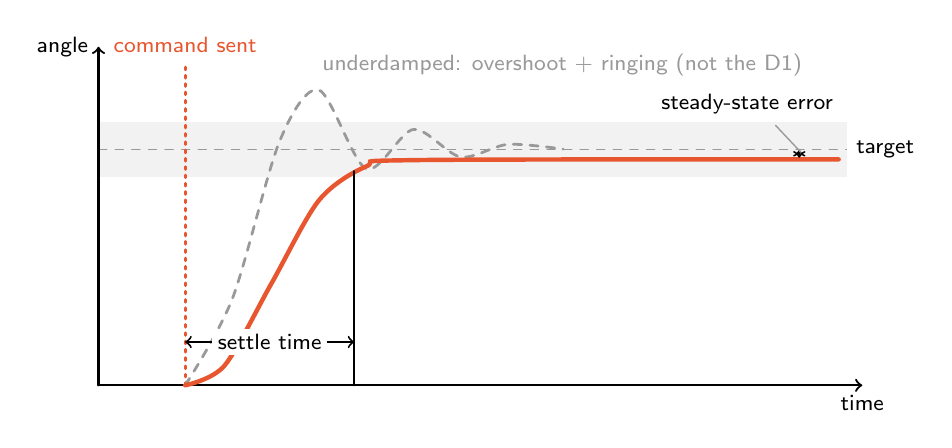
\begin{tikzpicture}[x=1cm,y=1cm,font=\footnotesize\sffamily,line cap=round]
  % settle band around target (target = 3.0, band +-0.35 drawn)
  \fill[codebg] (0.9,2.65) rectangle (10.4,3.35);
  \draw[rulegray,dashed] (0.9,3) -- (10.4,3) node[anchor=west,black]{target};
  % axes
  \draw[->,line width=0.8pt] (0.9,0) -- (10.6,0) node[anchor=north]{time};
  \draw[->,line width=0.8pt] (0.9,0) -- (0.9,4.3) node[anchor=east]{angle};
  % command instant
  \draw[accentorange,dotted,line width=1pt] (2,0) -- (2,4.1);
  \node[accentorange,anchor=south] at (2,4.1) {command sent};
  % underdamped ghost
  \draw[rulegray,line width=1pt,dashed] plot[smooth] coordinates
    {(2,0) (2.6,1.1) (3.2,3.1) (3.7,3.75) (4.3,2.75) (4.9,3.25)
     (5.5,2.9) (6.1,3.06) (6.8,3)};
  \node[rulegray,anchor=south west] at (3.62,3.8)
    {underdamped: overshoot + ringing (not the D1)};
  % overdamped response
  \draw[accentorange,line width=1.6pt] plot[smooth] coordinates
    {(2,0) (2.5,0.25) (3.1,1.3) (3.7,2.35) (4.3,2.78) (4.9,2.86)
     (10.3,2.87)};
  % settle time marker: first enters band and stays
  \draw[line width=0.7pt] (4.15,0) -- (4.15,2.72);
  \draw[<->,line width=0.7pt] (2,0.55) -- (4.15,0.55)
    node[midway,fill=white,inner sep=2pt]{settle time};
  % steady-state error
  \draw[<->,line width=0.7pt] (9.8,2.89) -- (9.8,2.99);
  \node[anchor=south east] at (10.35,3.32) {steady-state error};
  \draw[line width=0.5pt,rulegray] (9.82,2.96) -- (9.5,3.3);
\end{tikzpicture}
\caption{Anatomy of a step response. The command jumps at the dotted
line; the joint (solid curve) ramps toward the target and rests slightly
short of it --- the steady-state error. Settle time is measured to where
the curve enters the shaded $\pm0.5^\circ$ band and stays. The dashed
curve shows the underdamped alternative the D1 never exhibits: crossing
the target and oscillating.}
\label{fig:stepanatomy}
\end{figure}

Per joint, the procedure was: log a 5\,s baseline at zero; step to
$+10^\circ$, log 12\,s; back to zero; step to $-10^\circ$; step to
$+30^\circ$; then log 5\,s at zero again to confirm clean return. Seven
joints, three steps each, plus baselines --- 21 step tests and 14 static
logs, all automated by \code{run\_phase2.sh} in about eight minutes.

\subsection{The logger-first pattern}

The orchestration detail that makes the data good:

\codefile{experiments/run\_phase2.sh (core pattern)}
\begin{lstlisting}
python3 log_joints.py --duration 12 --label step_j2_pos10 &
sleep 2                       # capture the "before" state
echo "0 0 10 0 0 0 0" | ./joint_commander
wait                          # logger finishes its 12 s
\end{lstlisting}

The logger starts \emph{two seconds before} the command. Every CSV
therefore contains the pre-step baseline, the transient, and the settled
tail --- the complete story, with no guessing about when the step
happened. This pattern recurs in Phase 3's sequence runner.

\section{The results}

Full numbers live in \code{experiments/PHASE2\_RESULTS.md}; the analysis
was produced by \code{plot\_phase2.py} from 45 CSVs in
\code{logs/phase2/}. Figure~\ref{fig:phase2steps} shows the entire
campaign on one page --- worth a minute of study before reading the
numbers, because every finding below is visible in it.

\begin{figure}[p]
\centering
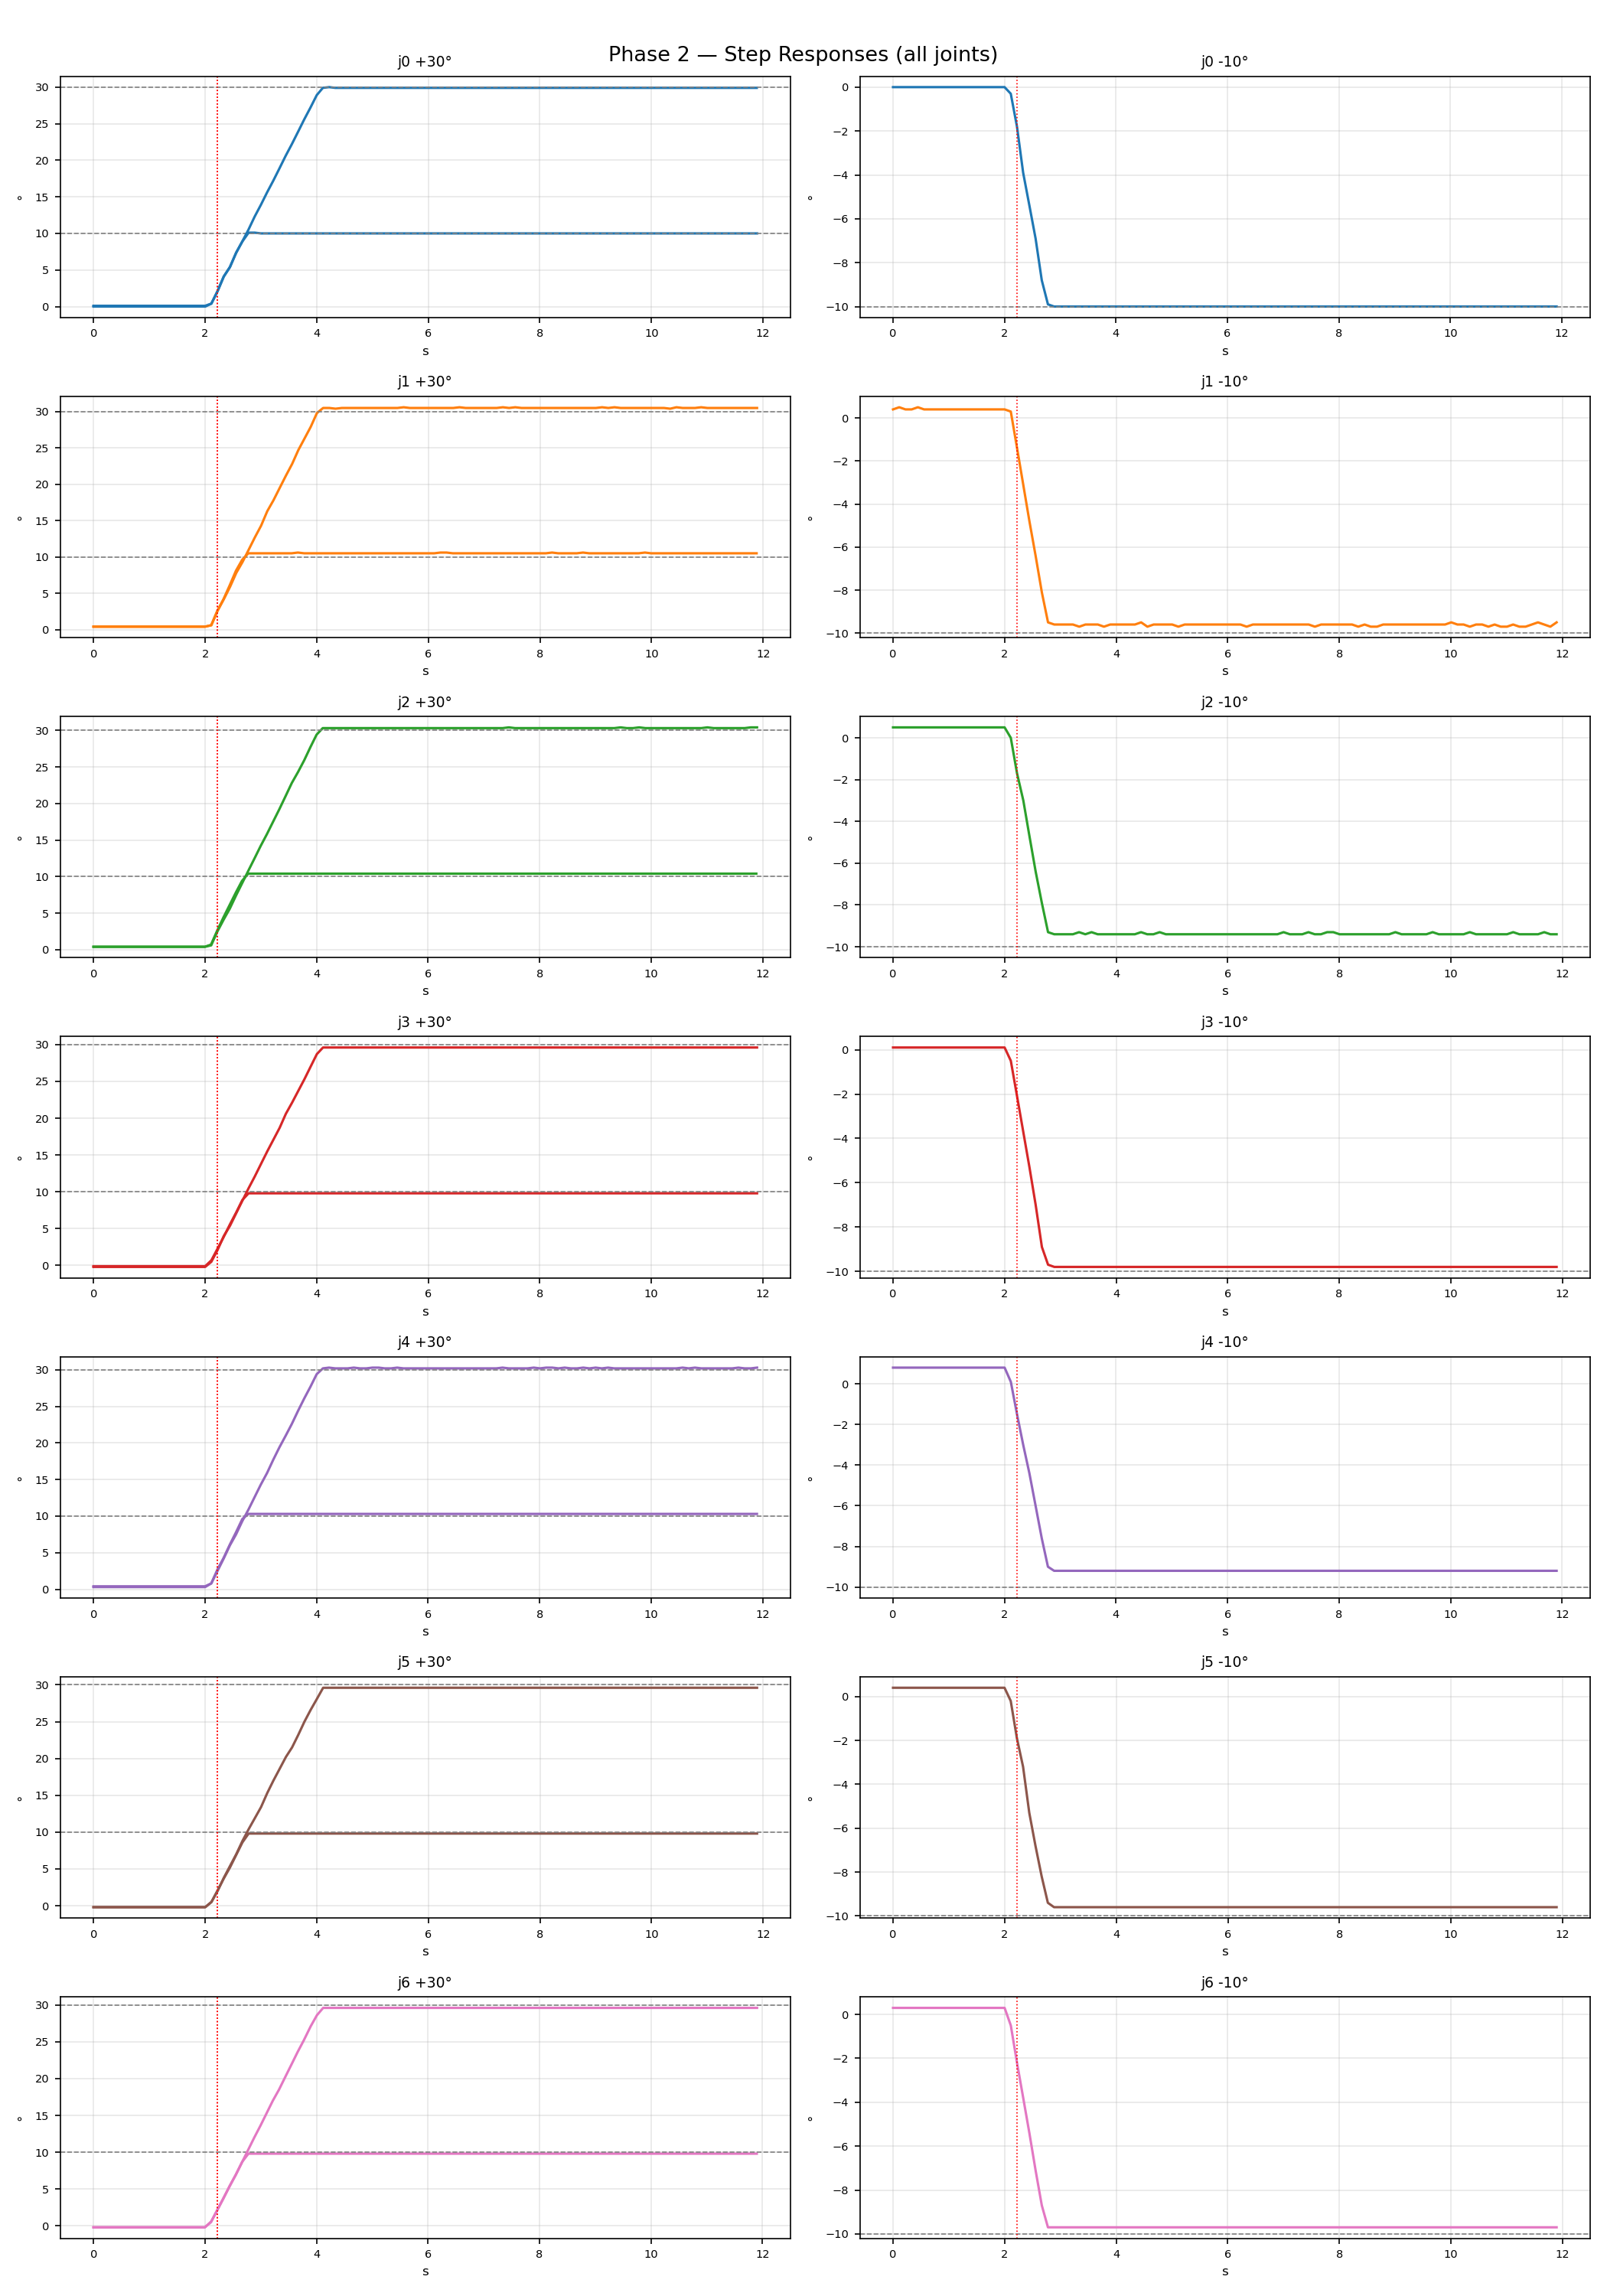
\includegraphics[width=\textwidth,height=0.92\textheight,keepaspectratio]{../logs/phase2/summary_step_responses.png}
\caption{All Phase 2 step responses, one row per joint. Left column:
$+30^\circ$ and $+10^\circ$ steps overlaid; right column: $-10^\circ$.
The red dotted line marks the moment the command was sent (2\,s into
each log --- the logger-first pattern); gray dashed lines are the
targets. Every trace approaches its target without crossing it
(overdamped), and the deadband finding is visible to the naked eye: in
the right column, j2 and j4 settle clearly short of $-10^\circ$ while
j0 and j3 reach it.}
\label{fig:phase2steps}
\end{figure}

\subsection{Zero offsets}

Commanded to zero, joints read between $-0.2^\circ$ and $+0.4^\circ$
(j0 is a perfect $0.000$; j1, j2, j4 sit around $+0.4^\circ$). Small, but
systematic --- so they are recorded in \code{limits.py} as
\code{ZERO\_OFFSETS} and will be subtracted by any controller that needs
precision.

\subsection{Step response character}

\begin{itemize}
  \item \textbf{Settle time}: $\pm10^\circ$ steps settle in
    0.45--0.67\,s; $\pm30^\circ$ steps in 1.78--1.89\,s.
  \item \textbf{All responses are overdamped} --- no joint overshoots,
    ever. Practically, this means moves can be commanded back-to-back
    without waiting out oscillations, and a $60^\circ$ swing can be
    bounded by extrapolating settle time rather than fearing ring-out.
  \item \textbf{Steady-state error}: between $0.0^\circ$ and
    $0.8^\circ$ depending on joint and direction. j0 is the most accurate
    joint; j4 in the negative direction is the worst.
\end{itemize}

\begin{pktnote}
\textbf{Overdamped}, in control terms: the system approaches its target
without crossing it, like a door with a strong closer. The opposite ---
underdamped --- overshoots and oscillates. Overdamped is the friendly case
for safety, at the cost of some speed.
\end{pktnote}

\subsection{The deadband discovery}

The interesting finding: \textbf{j2 and j4 cannot reach small negative
targets}. Commanded to $-10^\circ$, j2 lands at $-9.40^\circ$ and j4 at
$-9.20^\circ$ (visible in Figure~\ref{fig:phase2steps}, right column).

\begin{pktpredict}
Two hypotheses fit a joint that stops short: \emph{mechanical friction}
--- the joint physically cannot quite get there --- and a
\emph{controller deadband} --- firmware deliberately stops driving once
the remaining error is small. Before reading on: what single, cheap
measurement would tell these two apart? Commit to an answer first.
\end{pktpredict}

The discriminating measurement is \textbf{repetition}. A five-trial
repeatability test (\code{test\_deadband.sh}) measured the spread of the
landing point across trials: \textbf{0.00$^\circ$} --- every single
time, exactly the same shortfall. That number does the diagnostic work:

\begin{itemize}
  \item \textbf{Mechanical friction} is messy --- it would scatter the
    landing point across trials.
  \item \textbf{A controller deadband} is exact --- firmware stops
    commanding torque once position error drops below a threshold, so the
    joint parks at precisely the same shortfall every time.
\end{itemize}

Zero spread means deadband, not damage: the arm's internal controller
gives up $0.60^\circ$ early on j2 and $0.80^\circ$ early on j4, in the
negative direction only. No hardware problem, and the fix is pure
software --- to land j2 at exactly $-10.0^\circ$, command
$-10.6^\circ$. These corrections are \code{NEG\_DEADBAND} in
\code{limits.py}.

\begin{pktnote}
``Firmware'' here is more approachable than the word suggests: the D1's
controller is a small Linux computer running Unitree's \code{marm\_*}
services, and per the official docs its driver source
(\code{marm\_code/src/}) is reachable over SSH. A future side-quest could
locate the position-error threshold in \code{marm\_control} and confirm
this deadband at its source. Until then, the measured correction table is
the contract.
\end{pktnote}

\subsection{Coupling}

None detected. With any single joint commanded, all others stayed inside
their zero-offset noise floor ($<0.1^\circ$). In the tested range the
joints are mechanically independent --- which licenses the multi-joint
work of Phase 3.

\section{Recap --- what Phase 2 bought}

A correction table (offsets + deadband), trust in the servo controller
(overdamped, repeatable), timing constants for everything that follows,
and a demonstrated method: measure, hypothesize, re-measure to
discriminate.

\section*{Summary}
\addcontentsline{toc}{section}{Summary}

Seven joints characterized by automated step-response testing. The arm is
accurate to better than a degree, never overshoots, and hides one firmware
quirk --- a negative-direction deadband on j2 and j4 --- now documented
and correctable. Phase 3 builds on exactly these numbers.

\begin{pktcheck}
  \item From a step-response curve, define settle time, overshoot, and
    steady-state error --- then sketch the curve from memory and mark
    all three (compare with Figure~\ref{fig:stepanatomy}).
  \item Every D1 joint is overdamped. What practical freedom does that
    buy when commanding moves back-to-back?
  \item A five-trial repeat of the j2 $-10^\circ$ step measured a spread
    of $0.00^\circ$. Walk the logic: why does \emph{zero} spread rule
    out friction and implicate firmware?
  \item Why does every log start two seconds \emph{before} the command
    is sent?
  \item \code{ZERO\_OFFSETS} and \code{NEG\_DEADBAND} both live in
    \code{limits.py}. When must a controller apply each?
\end{pktcheck}

% =============================================================================
% CHAPTER
% =============================================================================

\chapter{Phase 3 --- The Safe Envelope}\label{ch:phase3}

Phase 2 moved one joint at a time. Phase 3 moves all of them, and its
product is a contract: \code{limits.py}, the per-joint bounds inside which
every future phase --- IK included --- is allowed to operate. This chapter
explains the pose set, the sequence experiment, and the path-dependence
analysis that decides whether the envelope can be trusted.

\section{The question Phase 3 answers}

Before an IK solver is allowed to pick arbitrary joint combinations, two
things must be established empirically:

\begin{enumerate}
  \item \textbf{Reachability without harm}: a set of multi-joint poses,
    spanning every joint in both directions, that the arm reaches without
    strain, odd sounds, or collision.
  \item \textbf{Path independence}: the arm lands in the \emph{same
    place} for a given pose regardless of where it came from. If arriving
    at \code{reach\_3} from \code{zero} gives a different settled position
    than arriving from \code{reach\_4}, then position commands don't mean
    what they appear to mean, and everything downstream inherits the
    ambiguity.
\end{enumerate}

Path dependence in a real arm comes from physical effects: gear backlash
(slack that loads differently depending on approach direction), stiction,
and gravity sag that varies with configuration. The Phase 2 deadband is a
small example already in hand --- approach direction changing the landed
position.

\section{The pose set and its coverage}

The nine poses in \code{poses.py} (shown in Chapter~\ref{ch:toolkit}) were designed
around a coverage argument, all inside the $\pm45^\circ$ conservative
ceiling:

\begin{itemize}
  \item \textbf{zero, reach\_1 \ldots\ reach\_4}: a progression of
    increasingly extended reach postures, j1 roughly doubling per step
    ($-5$, $-10$, $-20$, $-30^\circ$) while j2 rises to $+30^\circ$ and
    j4 to $+20^\circ$. \code{reach\_2} is the known-good anchor the
    remaining poses hold.
  \item \textbf{yaw\_left / yaw\_right}: base joint j0 at $\pm30^\circ$,
    with the arm held in the \code{reach\_2} anchor posture.
  \item \textbf{wrist\_open / wrist\_closed}: wrist rotations j3 and j5 at
    $\pm25^\circ$ with mirrored signs, same posture. The gripper j6
    is exercised alongside them --- but only on its documented side:
    \code{wrist\_open} opens it to 25, \code{wrist\_closed} brings it back
    to 0. An earlier draft of the pose set commanded j6 to $-25$, which
    is outside the gripper's 0--65\,mm stroke entirely; Phase~2 showed
    the controller tolerates negative j6, but a tolerated
    out-of-range command is not a safe envelope, so
    \code{limits.py} now pins j6 to $[0, 45]$.
\end{itemize}

Known gaps, on purpose: j1 positive and j2/j4 negative are unexercised,
because the original pose set only moved those joints one way and the
untested directions may drive the arm toward the table or itself. The
envelope those directions get is whatever Phase 2's single-joint
$-10^\circ$ tests justify, until poses are added deliberately.

\section{run\_sequence.py --- the experiment driver}

The Phase 3 procedure --- send each pose, log 10\,s, visually confirm,
repeat in multiple orders --- is automated by
\code{experiments/run\_sequence.py}. The orderings are \emph{derived} from
the pose dict, so new poses join the experiment automatically:

\codefile{experiments/run\_sequence.py}
\begin{lstlisting}[style=pktpython]
_ALL = list(poses)
ORDERS = {
    "A": _ALL,                    # as defined (starts at zero)
    "B": _ALL[::-1],              # reversed (ends at zero)
    "C": _ALL[::2] + _ALL[1::2],  # interleaved: bigger jumps
}
\end{lstlisting}

Within a sequence, poses run \textbf{back-to-back} --- deliberately not
re-zeroing between steps, because the pose-to-pose transitions are exactly
what path-dependence testing needs. The arm re-zeros and settles only
between sequences, so each ordering starts from the same state.

Each step reuses the logger-first pattern from Phase 2 and then puts a
human in the loop:

\begin{lstlisting}[style=pktpython]
proc, csv_path = start_logger(label)   # 2 s baseline first
time.sleep(PRE_WAIT)
send_pose(angles)                      # validated, then sent
proc.communicate()                     # 10 s observation
note = input("Strain / odd sound / collision? "
             "Enter = clean, or describe: ").strip()
\end{lstlisting}

The observation prompt is not decoration --- it implements the Phase 3
safety rule. A typed note is recorded in the run's markdown log and offers
an abort.

\begin{pktpredict}
The operator hits Ctrl-C mid-sequence because something sounded wrong.
Should the runner drive the arm back to zero automatically? Decide ---
and note your reasoning --- before reading on.
\end{pktpredict}

\begin{pktimportant}
On abort or Ctrl-C the arm is deliberately \textbf{left where it is}. An
automatic return-to-zero sounds helpful, but if the arm has just collided
with something, driving it back through the obstacle makes things worse.
The operator inspects, then re-zeros manually with
\code{python experiments/send\_pose.py zero}.
\end{pktimportant}

Every run --- complete or aborted --- writes
\code{logs/phase3/sequence\_log\_<stamp>.md}: one row per step with pose,
angles, CSV filename, and the operator's observation. That file is the
phase's required ``sequence log'' artifact.

\section{analyze\_sequences.py --- the verdict}

After the runs, \code{analyze\_sequences.py} reads every step CSV, takes
the \textbf{mean of the final two seconds} as the settled position (safe
because Phase 2 showed worst-case settling under 2\,s, leaving $\ge$ 8\,s
of settled data in each 10\,s observation), and groups by pose: where did
\code{reach\_3} land when reached via order A, B, and C?

\begin{pktpredict}
The analyzer needs a pass/fail rule: how much may a pose's settled
position vary across the three orderings before it counts as path
dependence? Phase 2 measured steady-state errors up to $0.8^\circ$ and
deadbands of $0.6$--$0.8^\circ$. Propose a threshold from those numbers
before reading the one the project chose.
\end{pktpredict}

The decision rule: per joint, the \textbf{spread} (max minus min across
orderings) must stay within $1.0^\circ$. The threshold comes from Phase 2,
not from taste --- steady-state errors up to $0.8^\circ$ and deadbands of
$0.6$--$0.8^\circ$ are already known repeatability, so only spread beyond
that indicates a path effect. Anything flagged gets re-run before
\code{limits.py} is touched, to rule out one-off noise.

\begin{pkttip}
The analyzer was validated before ever seeing real data, by feeding it
synthetic CSVs with a known $2^\circ$ path-dependence injected on one
joint of one pose. It flagged exactly that joint and nothing else. Test
your instruments before trusting what they say about the world.
\end{pkttip}

\section{Exit criteria}

Phase 3 closes when: the poses are defined and each has been executed and
visually confirmed clean; the three orderings have run; the analyzer
reports all spreads $\le 1.0^\circ$ (or the exceptions are understood and
documented); and \code{limits.py} is committed with its PROVISIONAL note
replaced by confirmed bounds. Then the tag \code{phase3-envelope-frozen}
is laid down and the envelope stops being negotiable.

\section*{Summary}
\addcontentsline{toc}{section}{Summary}

Phase 3 turns ``the arm can reach these poses'' into a tested, frozen
contract. Nine poses cover every joint, three orderings probe path
dependence, a human confirms each step, and a validated analyzer makes the
call against a threshold derived from Phase 2 data. What comes out is the
single file every future phase imports before moving metal.

\begin{pktcheck}
  \item Phase 3 answers two empirical questions before any IK is
    allowed. What are they?
  \item Within a sequence, poses run back-to-back with no re-zeroing.
    Why is that a feature rather than sloppiness?
  \item On abort or Ctrl-C, the arm is left where it is. Reconstruct the
    argument for why auto-zeroing would be worse.
  \item The path-dependence threshold is a $1.0^\circ$ spread. Where
    does that number come from --- and why would $0.3^\circ$ have been
    a bad choice?
  \item What was done to \code{analyze\_sequences.py} before it ever saw
    real data, and what principle does that illustrate?
\end{pktcheck}

% =============================================================================
% CHAPTER
% =============================================================================

\chapter{The Road Ahead}\label{ch:road}

Everything so far has been careful plumbing and measurement. The phases
ahead are where the robotics theory arrives. This chapter previews each
one --- what it builds, the core idea in plain terms, and what to read ---
so the mathematics never lands cold.

\section{What to be comfortable with first}

The common foundation for Phases 4--6 is linear algebra, used concretely:

\begin{itemize}
  \item \textbf{Matrix multiplication as composition}: chaining
    transforms means multiplying matrices, in order. Order matters.
  \item \textbf{Rotation matrices} ($3\times3$, orthonormal) and
    \textbf{homogeneous transforms} ($4\times4$, rotation plus
    translation --- the set called SE(3)).
  \item \textbf{Cross products} and their matrix form (the ``skew''
    matrix), which is how rotation axes enter the algebra.
  \item \textbf{Radians} internally, always; degrees only at the
    tool boundary.
  \item \textbf{NumPy fluency}: \code{@}, broadcasting,
    \code{np.linalg}.
\end{itemize}

The theory source for the whole arc is \textit{Modern Robotics} by Lynch
\& Park (free PDF online). Each phase below names its chapter.

\section{Phase 4 --- forward kinematics}

\textbf{The question}: given seven joint angles, where is the
end-effector in 3D space?

The implementation uses the \textbf{Product of Exponentials} (POE)
formula rather than the older Denavit--Hartenberg tables. The intuition:
each joint is a hinge in space, described by a \textbf{screw axis} --- a
6-vector $S = [\omega, v]$ bundling the rotation axis and where it sits.
Rotating joint $i$ by $\theta_i$ transforms everything beyond it by the
matrix exponential $e^{[S_i]\theta_i}$. Chain all seven, close with $M$
(the end-effector pose at zero configuration), and that is FK:

\begin{lstlisting}
T(theta) = exp([S1] th1) exp([S2] th2) ... exp([Sn] thn) M
\end{lstlisting}

The screw axes and $M$ come from the D1's URDF file (already in the
repository), parsed with Python's XML tools. Validation is physical: tape
a grid to the table, command three known configurations, and require the
prediction to land within 2\,cm of where the arm's tip actually is ---
which is why Phase 2's zero offsets and Phase 3's safe poses had to come
first. \emph{Read: Lynch \& Park Chapter 4 (and Chapter 3 for Rodrigues'
rotation formula).}

\section{Phase 5 --- Jacobians and differential IK}

\textbf{The question}: to nudge the end-effector 1\,cm in $+x$, how
should the joints move?

The \textbf{Jacobian} $J(\theta)$ is the matrix that maps joint
velocities to end-effector velocity at the current configuration ---
column $i$ is joint $i$'s screw axis re-expressed at the current pose.
Differential IK inverts the map. Because $J$ can be non-square and
near-singular, the inversion uses \textbf{damped least squares},
$J^{T}(JJ^{T}+\lambda^{2}I)^{-1}$, which trades a little accuracy for not
exploding near singular poses (configurations where some direction of
motion is momentarily impossible, like a fully stretched arm being asked
to extend further). Hardware target: a commanded 1\,cm Cartesian step
lands within 5\,mm. \emph{Read: Lynch \& Park Chapter 5.}

\section{Phase 6 --- numerical IK}

\textbf{The question}: given a target pose, what joint angles reach it?

There is no closed-form answer for a general arm; instead, iterate
differential IK Newton-style --- compute the pose error as a twist
(via the matrix log, the inverse of Phase 4's exponential), take a
damped step, clamp to \code{LIMITS}, repeat until converged. The
engineering is in the failure handling: convergence tolerances split
between rotation and translation, retry seeds when iteration stalls, and
an automated suite of 200 random reachable targets with a $\ge 90\%$
success requirement. \code{limits.py} appears here in its final role:
the clamp inside every IK step. \emph{Read: Lynch \& Park Chapter 6.}

\section{Phase 7 --- ROS 2}

ROS 2 replaces the stdin/stdout bridge with the industry-standard
middleware --- which is DDS underneath, the same technology the D1
already speaks. The vocabulary: a \textbf{node} is a process that does
one thing; \textbf{topics} are pub/sub streams (a
\code{joint\_state\_publisher} node will publish the arm's angles on
\code{/joint\_states}); \textbf{services} are request/reply (FK becomes a
service); \textbf{actions} are long-running goals with feedback
(trajectories, later). The first milestone is RViz showing the URDF model
tracking the real arm live. The repository's \code{ROS2/cheatsheet.md}
holds the working notes.

ROS 2 distributions pair with Ubuntu LTS releases; on this project's
Ubuntu 26.04 the matching distribution is \textbf{ROS 2 Lyrical Luth}.
Install the official binary packages from docs.ros.org --- never build
ROS from source for this --- plus
\code{python3-colcon-common-extensions}. If the workstation OS ever
changes, the distribution changes with it; everything conceptual in this
section survives that swap untouched. \emph{Read: the official
docs.ros.org beginner tutorials, all of them --- one day that saves a
week.}

\section{Phases 8--11 --- trajectories, simulation, perception, capstone}

\textbf{Trajectories (Phase 8)}: replace ``go to pose'' with a timed
path. Cubic time scaling $s(t)=3s^2-2s^3$ (zero velocity at endpoints) or
quintic (zero acceleration too) shapes the motion; an executor streams
waypoints through the commander. Gravity compensation is empirical: hold
poses, measure droop versus angle, fit a $k\sin\theta$ correction ---
the same measure-then-model pattern as Phase 2.

\textbf{Simulation (Phase 9)}: load the URDF into MuJoCo, require FK
agreement within 5\,mm, then run identical trajectories in sim and on
hardware and document the gap.

\textbf{Perception (Phase 10)}: calibrate a webcam
(reprojection error $<1$\,px), detect ArUco markers for 6-DOF object
pose, transform camera coordinates into the robot base frame, publish on
a ROS 2 topic.

\textbf{Capstone (Phase 11)}: chain everything --- detect, IK, plan,
execute, place --- and measure it honestly: 20 trials, success rate and
grasp-position error with mean and standard deviation, target
$\ge 15/20$.

\section*{Summary}
\addcontentsline{toc}{section}{Summary}

The arc runs measurement $\rightarrow$ model $\rightarrow$ control
$\rightarrow$ integration: characterize the joints, learn where the
end-effector is (FK), learn how to move it (Jacobians, IK), industrialize
the plumbing (ROS 2), make motion smooth (trajectories), and close the
loop with eyes (perception). Every stage stands on the measured
foundations of Phases 2 and 3 --- which is the whole argument for having
built them carefully.

\begin{pktcheck}
  \item Forward kinematics answers what question, and the Product of
    Exponentials formula chains what quantities to answer it?
  \item The Jacobian maps what to what --- and why does inverting it
    need damped least squares rather than a plain inverse?
  \item Numerical IK is described as iterating two pieces built earlier.
    Which two, and what keeps each step inside the safe envelope?
  \item Why is ROS 2 an unusually natural fit for this particular arm?
\end{pktcheck}

% =============================================================================
% APPENDIX
% =============================================================================

\appendix

% Appendix chapters: letter instead of number
\titleformat{\chapter}[display]
  {\headingfont\bfseries}
  {\filright\fontsize{40}{40}\selectfont\color{accentorange}Appendix \thechapter}
  {6pt}
  {\Huge\bfseries\filright}

\chapter{Quick Reference}

Everything in this appendix is the perishable layer --- exact names,
versions, and numbers as of this edition's repository revision (see the
colophon). When something here disagrees with the repository, trust the
repository and update this appendix.

\section{Environment}

\begin{itemize}
  \item \textbf{OS}: Ubuntu 26.04 LTS (Resolute Raccoon)
  \item \textbf{ROS 2}: Lyrical Luth (Phase 7 onward; binary install)
  \item \textbf{DDS}: Eclipse CycloneDDS via \code{unitree\_sdk2}
  \item \textbf{Python}: system Python 3; NumPy/matplotlib/pandas for
    analysis
  \item \textbf{Network}: robot \code{192.168.123.100}, host
    \code{192.168.123.10} (profile \code{d1-robot})
\end{itemize}

\section{Bring-up and smoke test}

\begin{lstlisting}
$ ./setup.sh                      # fresh machine or new adapter
# power the arm, wait 60-90 s, then from d1_sdk/build/:
$ ./get_arm_joint_angle           # verify telemetry FIRST
$ ./joint_enable_control          # lock joints
$ ./arm_zero_control              # move to zero posture
\end{lstlisting}

\section{Everyday commands}

\begin{lstlisting}
# send a named pose or raw angles (validated against limits.py)
$ python experiments/send_pose.py zero
$ python experiments/send_pose.py 0 -30 30 0 20 0 0

# log telemetry to CSV
$ python experiments/log_joints.py --duration 12 --label mytest

# raw one-liner, bypassing Python (no limit checks -- careful)
$ echo "0 0 0 0 0 0 0" | d1_sdk/build/joint_commander
\end{lstlisting}

\section{Phase experiment workflows}

\begin{lstlisting}
# Phase 2: full characterization (~8 min) and analysis
$ bash experiments/run_phase2.sh
$ python3 experiments/plot_phase2.py --summary --table
$ bash experiments/test_deadband.sh        # j2/j4 recheck

# Phase 3: sequence runs and path-dependence verdict
$ python experiments/run_sequence.py        # or --only B
$ python experiments/analyze_sequences.py
\end{lstlisting}

\section{File map}

\begin{itemize}
  \item \code{experiments/poses.py} --- named poses (degrees on
    j0--j5; j6 is gripper stroke, $\geq 0$).
  \item \code{experiments/limits.py} --- \code{LIMITS},
    \code{ZERO\_OFFSETS}, \code{NEG\_DEADBAND}. The contract.
  \item \code{experiments/send\_pose.py} --- the only path to the robot;
    validates first.
  \item \code{experiments/log\_joints.py} --- telemetry to CSV;
    \code{--duration}, \code{--label}, \code{--outdir}.
  \item \code{experiments/run\_sequence.py} /
    \code{analyze\_sequences.py} --- Phase 3 driver and verdict.
  \item \code{experiments/PHASE2\_RESULTS.md} --- characterization
    numbers.
  \item \code{d1\_sdk/PROTOCOL.md} --- full JSON protocol reference.
  \item \code{logs/phaseN/} --- raw CSVs, immutable.
\end{itemize}

\section{Protocol crib sheet}

Envelope: \code{\{"seq": n, "address": a, "funcode": f, "data":
\{...\}\}}. Addresses: 1 = command (host $\rightarrow$ arm), 2 = state
feedback (arm $\rightarrow$ host, \code{seq}=10), 3 = command ack.
Commands on address 1: funcode 1 single joint, \textbf{2 all joints
(the one used here)}, 4/5 enable one/all, 6 power, 7 zero posture.
Feedback on address 2: funcode 1 angles at 10\,Hz, 3 status flags,
4 motor health. Acks on address 3: funcode 1 received-OK, 2 executed-OK.

\section{Measured constants (Phase 2)}

\begin{itemize}
  \item Settle: $\le 0.7$\,s for $10^\circ$ steps, $\le 1.9$\,s for
    $30^\circ$ steps; all joints overdamped, zero overshoot.
  \item Zero offsets: j1/j2/j4 $\approx +0.4^\circ$; j5/j6
    $\approx -0.2^\circ$; j0 exact.
  \item Deadband: j2 stops $0.60^\circ$ short and j4 $0.80^\circ$ short
    on negative targets --- perfectly repeatable, firmware, not damage.
  \item Coupling: none above the $0.1^\circ$ noise floor.
\end{itemize}

\section{Factory constants (D1-550 official spec)}

\begin{itemize}
  \item Range of motion: j0/j3/j5 $\pm135^\circ$; j1/j2/j4
    $\pm90^\circ$; j6 gripper 0--65\,mm stroke. \emph{Never approached
    in this project} --- the working envelope is \code{limits.py}.
  \item Torque: 3.3\,Nm (j0, j1); 1.7\,Nm (j2--j6). Payload 500\,g
    including gripper. Reach 550\,mm.
  \item Control cycle and telemetry rate: 10\,Hz. Power: 24\,V, 240\,W.
  \item Arm IP \code{192.168.123.100}; onboard Linux, SSH user
    \code{ubuntu}.
\end{itemize}

\section{References}

\begin{itemize}
  \item Official D1 services interface (protocol, specs, D1-T setup,
    multi-arm control):\\
    \url{https://support.unitree.com/home/en/developer/D1Arm_services}
  \item D1 SDK + sample programs (requires \code{unitree\_sdk2}):
    \code{d1\_sdk.zip} from Unitree's firmware CDN, linked from the page
    above. URDF and meshes: the ``Robotic Arm Download'' links on the
    same page (gripper version already vendored in this repository).
  \item \textit{Modern Robotics}, Lynch \& Park --- free PDF online;
    chapter map in Chapter~\ref{ch:road}.
  \item ROS 2 Lyrical Luth: \url{https://docs.ros.org}
\end{itemize}

% =============================================================================
% APPENDIX B — ANSWERS
% =============================================================================

\chapter{Answers}\label{app:answers}

Answers to each chapter's ``Check your understanding'' questions. If one
of yours came out wrong, the fix is not to memorize this page --- re-read
the section, then try the question again tomorrow. Spaced, repeated
retrieval is what makes it permanent.

\section{Chapter 1 --- The Project and the Plan}

\begin{enumerate}
  \item \code{j0}--\code{j5} are true rotations. \code{j6} drives the
    gripper: a 0--65\,mm claw stroke (prismatic jaws in the URDF)
    exposed through an angle-style channel.
  \item Raw logs are the project's evidence. Analysis scripts may read
    them and derive anything; they may never edit them --- immutability
    keeps every conclusion re-derivable from ground truth.
  \item j0 and j1. At extension, gravity loads the proximal joints
    hardest while everything from j2 outward runs on half the torque ---
    which shapes both the conservative envelope and Phase 8's gravity
    compensation target.
  \item C++ lives only in \code{d1\_sdk/}, experiments in
    \code{experiments/}, raw data in \code{logs/} (write-once). One
    small surface touches the robot, the science stays in Python, and
    the evidence cannot be quietly rewritten.
\end{enumerate}

\section{Chapter 2 --- From Box to First Motion}

\begin{enumerate}
  \item Telemetry (\code{./get\_arm\_joint\_angle}). A stream of servo
    lines proves network, DDS, and arm are alive --- you establish that
    you can \emph{hear} the arm before you ask it to move.
  \item The motion is executed by the arm's onboard controller, not by
    your process --- Ctrl-C only kills the sender. The stop is the power
    switch, which is why a hand stays within reach of it.
  \item A stale network-interface name compiled into the binaries (the
    names are MAC-derived and change with the adapter). Re-run
    \code{./setup.sh}: it re-detects, re-patches, and rebuilds.
  \item Phase 2 characterization. Zero offsets and deadbands are
    per-unit facts about one arm's servos and firmware, not facts about
    the D1 model.
\end{enumerate}

\section{Chapter 3 --- Talking to the Arm}

\begin{enumerate}
  \item \code{rt/arm\_Command}: host $\rightarrow$ arm, JSON commands.
    \code{arm\_Feedback}: arm $\rightarrow$ host, JSON status and
    acknowledgements. \code{current\_servo\_angle}: arm $\rightarrow$
    host, \code{PubServoInfo\_} structs at $\sim$10\,Hz.
  \item Address 1 = commands to the arm; address 2 = continuous state
    feedback; address 3 = per-command acknowledgements. Messages the arm
    volunteers use \code{seq = 10}; acks echo the command's own
    \code{seq}.
  \item Mode 0 is light smoothing for 10\,Hz streaming updates; mode 1
    is a trajectory-style move with heavy smoothing. This project sends
    mode 1.
  \item Binding to the correct network interface by name. Get it wrong
    and multicast discovery simply never happens: the program runs,
    nothing moves, and no error is printed.
\end{enumerate}

\section{Chapter 4 --- The C++/Python Bridge}

\begin{enumerate}
  \item Publish commands and subscribe to telemetry --- nothing else.
    Validation, logging, analysis, and experiment logic all live in
    Python.
  \item The arm's own servo controller holds the last commanded
    position. The commander is a messenger, not a supervisor, so it can
    exit the moment the message is sent.
  \item Its output is a line protocol: one reading per line, fixed field
    names, flushed per line. Python just reads lines and applies a
    regex.
  \item The boundary itself: C++ owns robot I/O, Python owns the math.
    Phase 7 swaps the transport (pipes for ROS 2 topics) without moving
    the intelligence.
\end{enumerate}

\section{Chapter 5 --- The Experiment Toolkit}

\begin{enumerate}
  \item Count check, limits check, binary-exists check, then the
    subprocess call. Everything that can fail cheaply fails before metal
    moves.
  \item Wall-clock row stamps let logs from different tools be
    correlated; \code{--duration} uses the monotonic clock because wall
    time can jump (NTP) and monotonic time cannot.
  \item Divergent private copies of the limits. With a single imported
    \code{LIMITS}, tightening \code{limits.py} instantly constrains
    every tool in the repository.
  \item The \code{reach} ladder varies extension (j1, j2, j4); the yaw
    and wrist poses hold the proven \code{reach\_2} anchor and vary only
    the joints under test. That is ``one variable per experiment''
    expressed as data design.
\end{enumerate}

\section{Chapter 6 --- Phase 2}

\begin{enumerate}
  \item Settle time: from the command until the response enters and
    stays inside the $\pm0.5^\circ$ band. Overshoot: crossing the target
    and coming back. Steady-state error: the gap between where it
    finally rests and the target. All three are marked in
    Figure~\ref{fig:stepanatomy}.
  \item With no overshoot there is no ring-out to wait for: moves can be
    commanded back-to-back, and bigger swings can be bounded by
    extrapolating settle time instead of fearing oscillation.
  \item Friction is physically messy, so it would scatter the landing
    point from trial to trial. A spread of exactly zero means a
    deterministic rule stops the motion at the same error every time ---
    a firmware threshold, not mechanics.
  \item So every CSV contains the pre-step baseline. When the step
    happened and what the state was beforehand are \emph{in the data},
    never reconstructed from memory.
  \item \code{ZERO\_OFFSETS} is subtracted whenever precise positioning
    matters, on every joint. \code{NEG\_DEADBAND} is applied additionally,
    only on j2/j4 and only when targeting negative angles.
\end{enumerate}

\section{Chapter 7 --- Phase 3}

\begin{enumerate}
  \item Reachability without harm (the poses can be reached with no
    strain, odd sound, or collision) and path independence (a pose's
    settled position does not depend on where the arm came from).
  \item The pose-to-pose transitions are the experiment: path dependence
    shows up \emph{between} poses. Re-zeroing after every step would
    erase exactly the evidence being collected.
  \item If the arm has just collided with something, automatically
    driving it back to zero drags it through the obstacle again. The
    operator inspects first and re-zeros deliberately.
  \item From Phase 2's measured repeatability: steady-state errors up to
    $0.8^\circ$ and deadbands of $0.6$--$0.8^\circ$ are already normal.
    A $0.3^\circ$ threshold would flag known-healthy servo behavior as
    path dependence and drown the analysis in false alarms.
  \item It was fed synthetic CSVs with a known $2^\circ$ path effect
    injected on one joint of one pose, and it flagged exactly that and
    nothing else. Test your instruments before trusting what they say
    about the world.
\end{enumerate}

\section{Chapter 8 --- The Road Ahead}

\begin{enumerate}
  \item FK answers ``given joint angles, where is the end-effector?''
    POE chains one matrix exponential $e^{[S_i]\theta_i}$ per joint ---
    each screw axis rotated by its angle --- closed by $M$, the
    end-effector pose at zero configuration.
  \item Joint velocities to end-effector velocity, at the current
    configuration. Near singular poses a plain inverse blows up; damped
    least squares trades a little accuracy for bounded, stable steps.
  \item The differential-IK step (Jacobian inversion) and the matrix log
    (pose error expressed as a twist), iterated Newton-style --- with
    every iterate clamped to \code{LIMITS}.
  \item ROS 2 is DDS underneath --- the same middleware the D1 natively
    speaks, so the arm and the framework already share a wire protocol
    family.
\end{enumerate}

\end{document}
